\documentclass[compress]{beamer}
\usepackage{ifthen,verbatim}

\title{Multiple Scattering in FastSim, \\ for Muon Alignment}
\author{Jim Pivarski}
\institute{Texas A\&M University}
\date{ 3 June, 2008}

\newcommand{\isnote}{}
\xdefinecolor{lightyellow}{rgb}{1.,1.,0.25}
\xdefinecolor{darkblue}{rgb}{0.1,0.1,0.7}

%% Uncomment this to get annotations
%% \def\notes{\addtocounter{page}{-1}
%%            \renewcommand{\isnote}{*}
%% 	   \beamertemplateshadingbackground{lightyellow}{white}
%%            \begin{frame}
%%            \frametitle{Notes for the previous page (page \insertpagenumber)}
%%            \itemize}
%% \def\endnotes{\enditemize
%% 	      \end{frame}
%%               \beamertemplateshadingbackground{white}{white}
%%               \renewcommand{\isnote}{}}

%% Uncomment this to not get annotations
\def\notes{\comment}
\def\endnotes{\endcomment}

\setbeamertemplate{navigation symbols}{}
\setbeamertemplate{headline}{\mbox{ } \hfill
\begin{minipage}{5.5 cm}
\vspace{-0.75 cm} \small
\end{minipage} \hfill
\begin{minipage}{4.5 cm}
\vspace{-0.75 cm} \small
\begin{flushright}
\ifthenelse{\equal{\insertpagenumber}{1}}{}{Jim Pivarski \hspace{0.2 cm} \insertpagenumber\isnote/\pageref{numpages}}
\end{flushright}
\end{minipage}\mbox{\hspace{0.2 cm}}\includegraphics[height=1 cm]{../cmslogo} \hspace{0.1 cm} \includegraphics[height=1 cm]{../tamulogo} \hspace{0.01 cm} \vspace{-1.05 cm}}

\begin{document}
\frame{\titlepage}

%% \begin{notes}
%% \item This is the annotated version of my talk.
%% \item If you want the version that I am presenting, download the one
%% labeled ``slides'' on Indico (or just ignore these yellow pages).
%% \item The annotated version is provided for extra detail and a written
%% record of comments that I intend to make orally.
%% \item Yellow notes refer to the content on the {\it previous} page.
%% \item All other slides are identical for the two versions.
%% \end{notes}

\begin{frame}
\frametitle{Why are we interested?}
\begin{itemize}\setlength{\itemsep}{0.3 cm}
\item Want to study track-based alignment procedures for muon system (tracker alignment group is interested, too)
\item CSA08 FullSim only allows us to test 1 and 10~pb$^{-1}$, but alignments from up to 100~pb$^{-1}$ are interesting for physics studies
\item In real life, we would align with all muons above a given $p_T$ cut, not just $W$ and $Z$ muons: prohibitive for FullSim (without a 10$\times$ CSA08!)
\item All the simulation needs to get right for alignment: 

residuals distributions on each alignable
\item Multiple scattering is essential!

(Factor of $N$ in stdev of chamber residual distribution fakes a factor of $1/N^2$ in statistics)
\end{itemize}
%% \hspace{-0.83 cm} \textcolor{darkblue}{\Large Outline2}
\end{frame}

\begin{frame}
\frametitle{Tracker-to-muon residuals: \only<1>{MB1}\only<2>{MB2}\only<3>{MB3}\only<4>{MB4}}
\only<1>{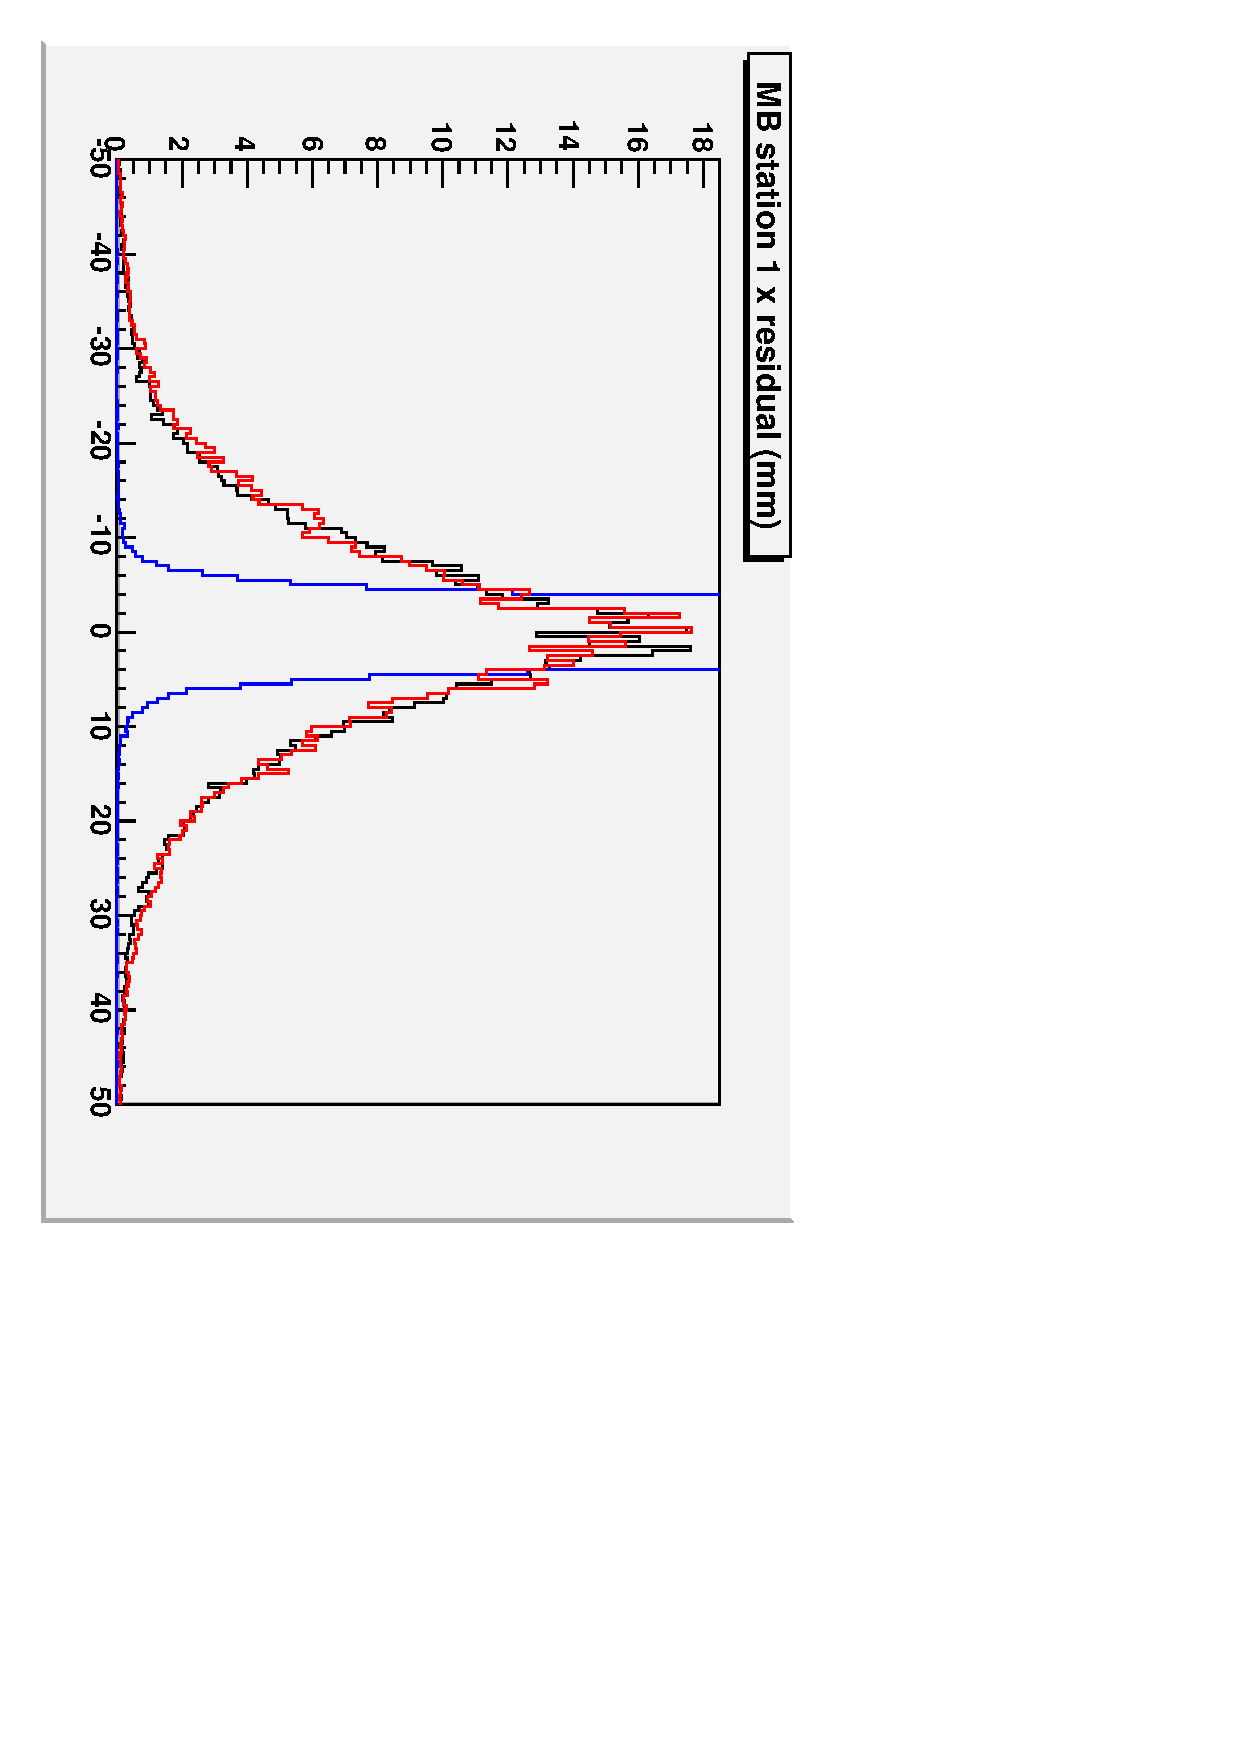
\includegraphics[height=\linewidth, angle=90]{xresid_mb1.pdf}}
\only<2>{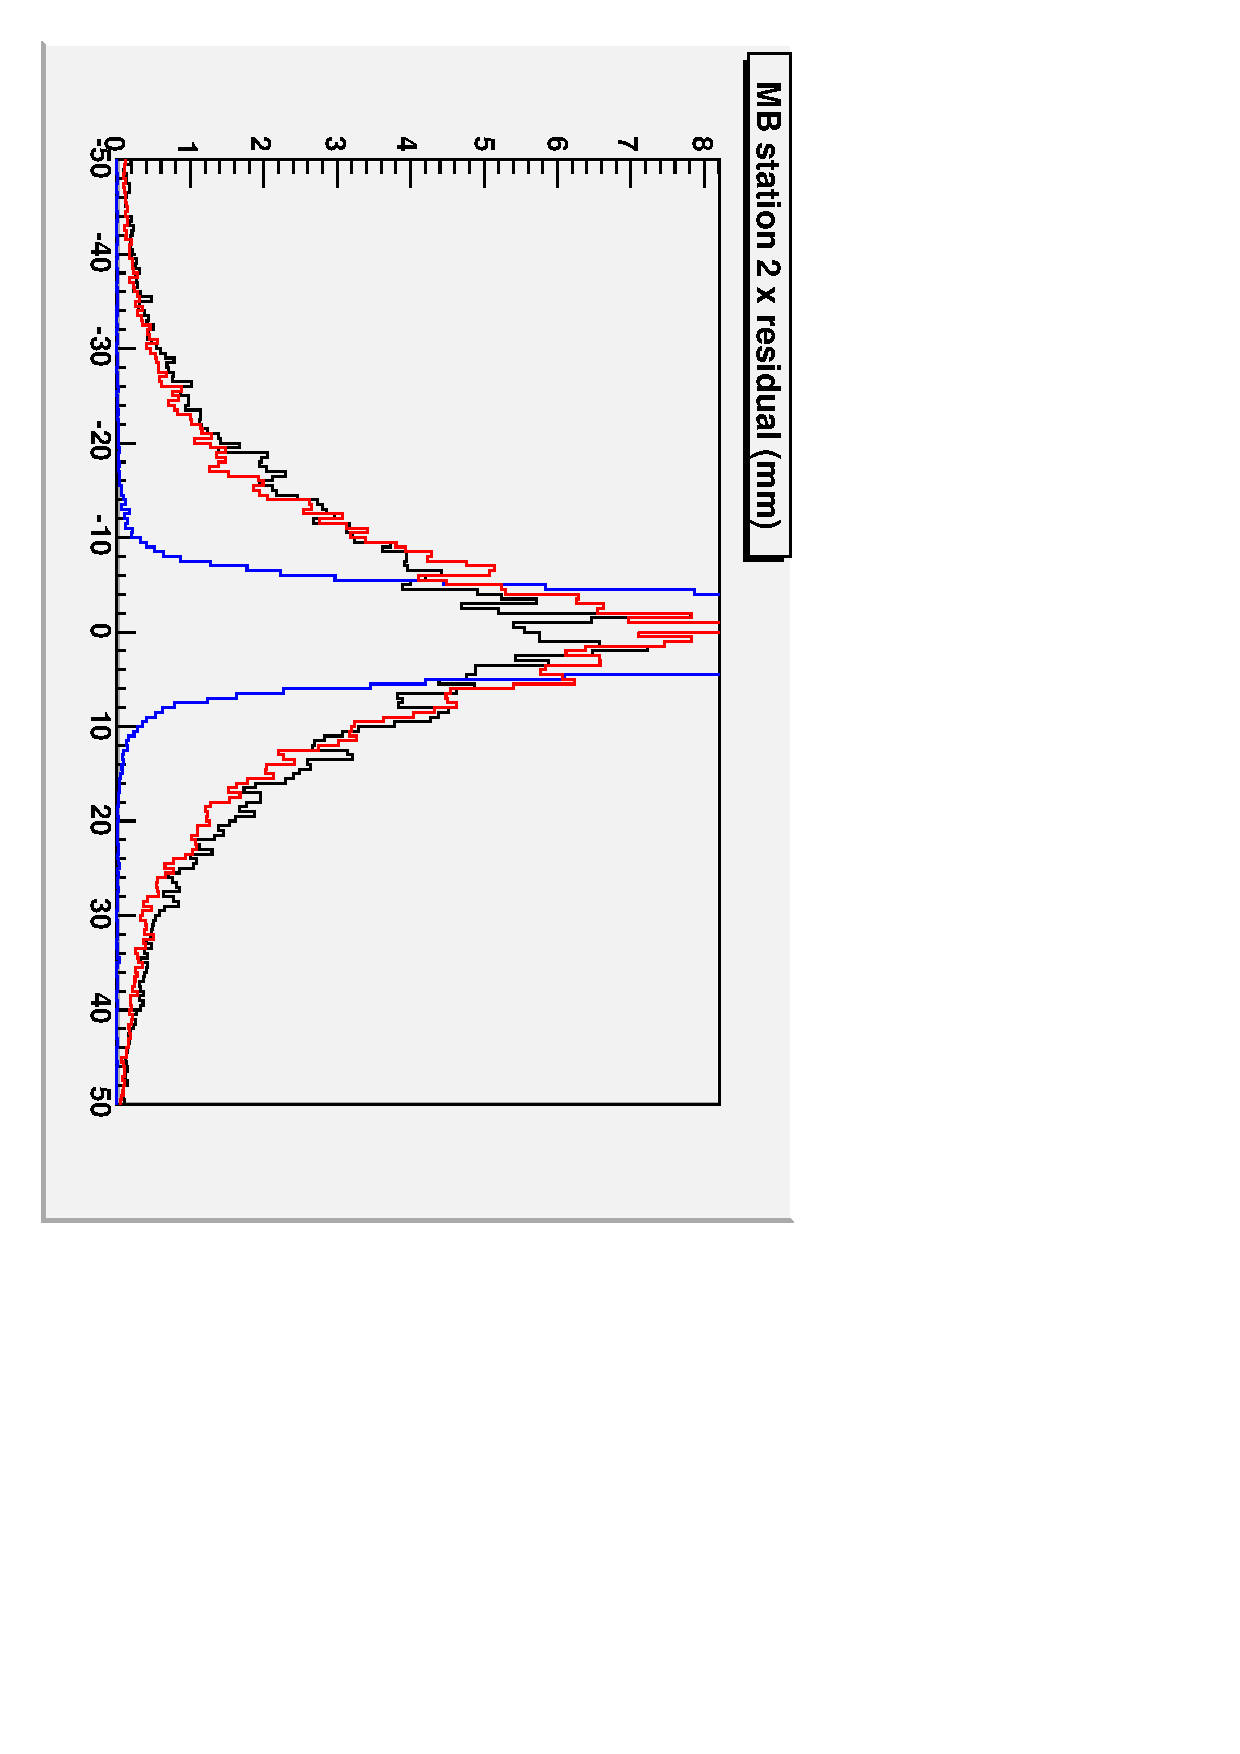
\includegraphics[height=\linewidth, angle=90]{xresid_mb2.pdf}}
\only<3>{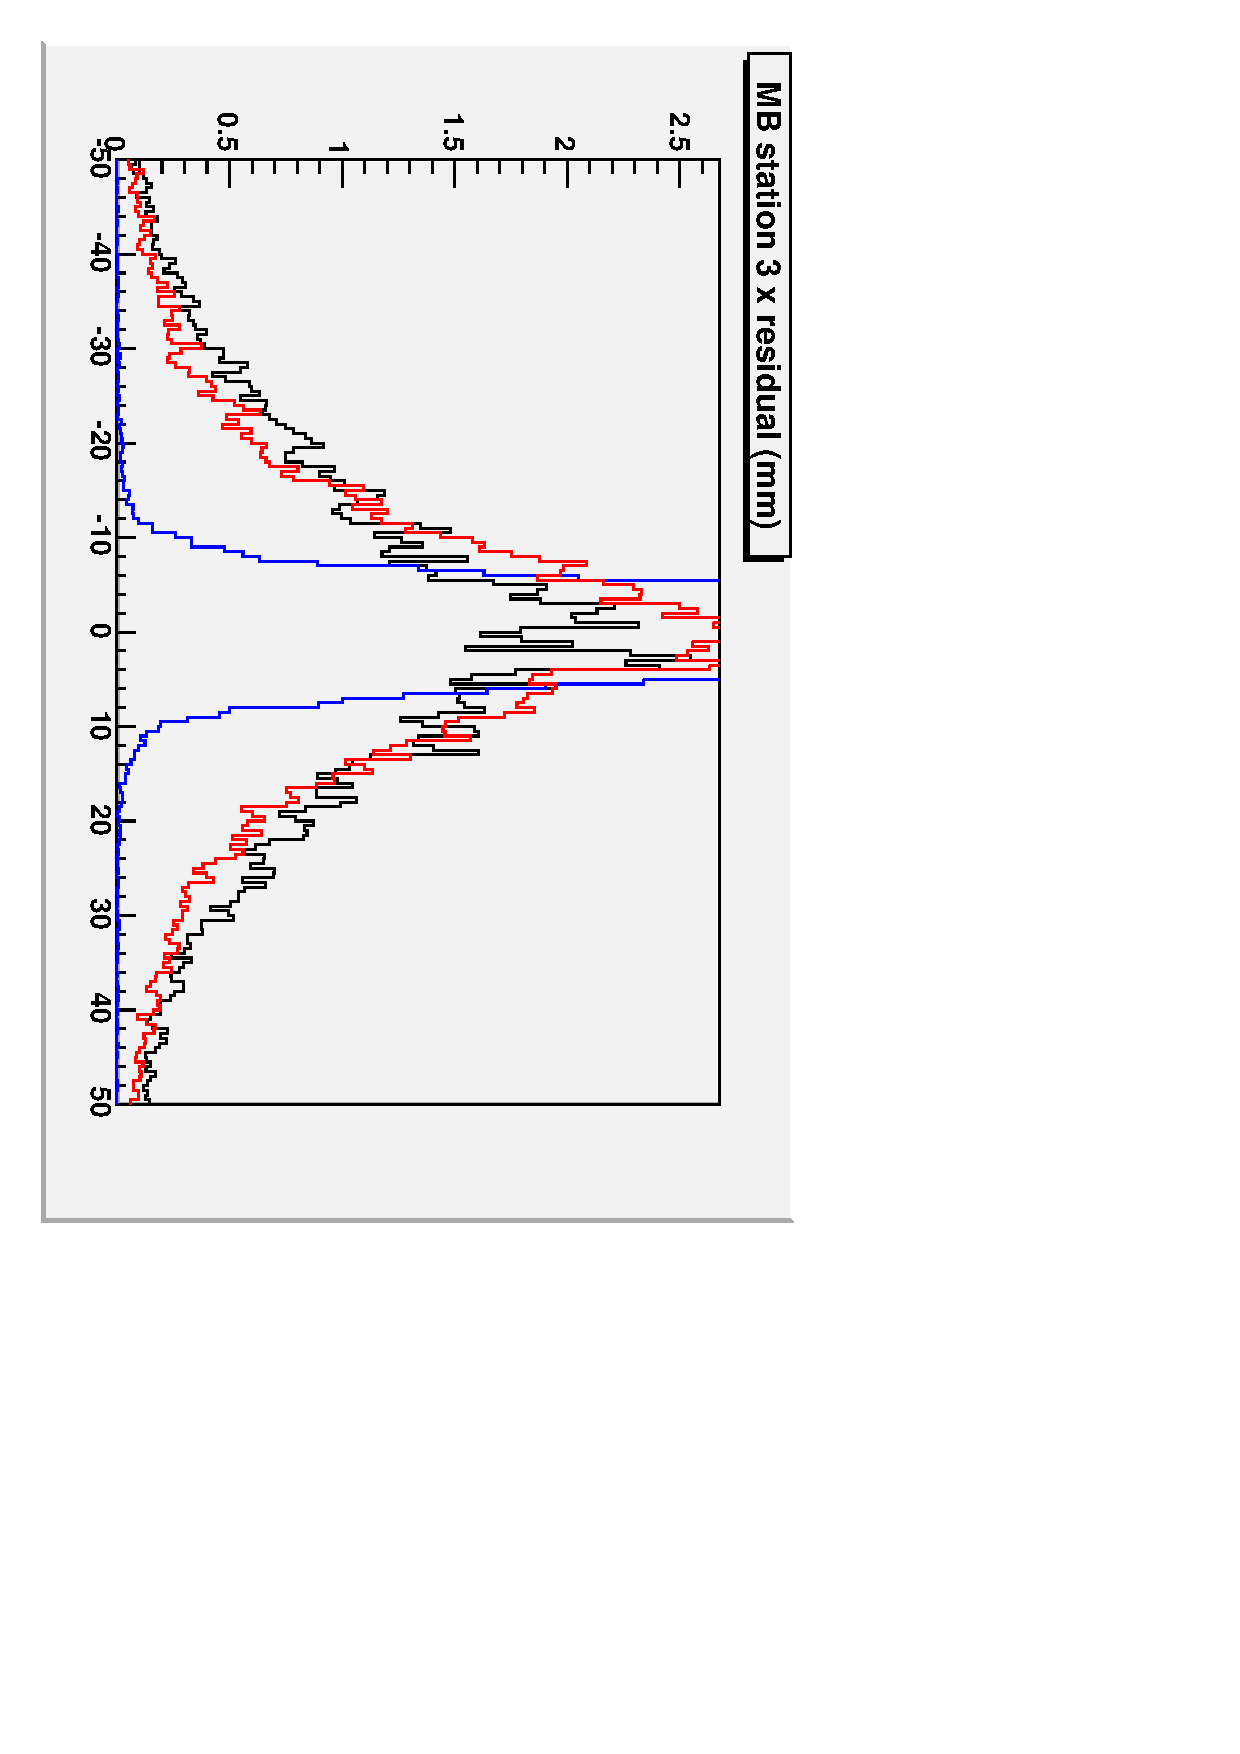
\includegraphics[height=\linewidth, angle=90]{xresid_mb3.pdf}}
\only<4>{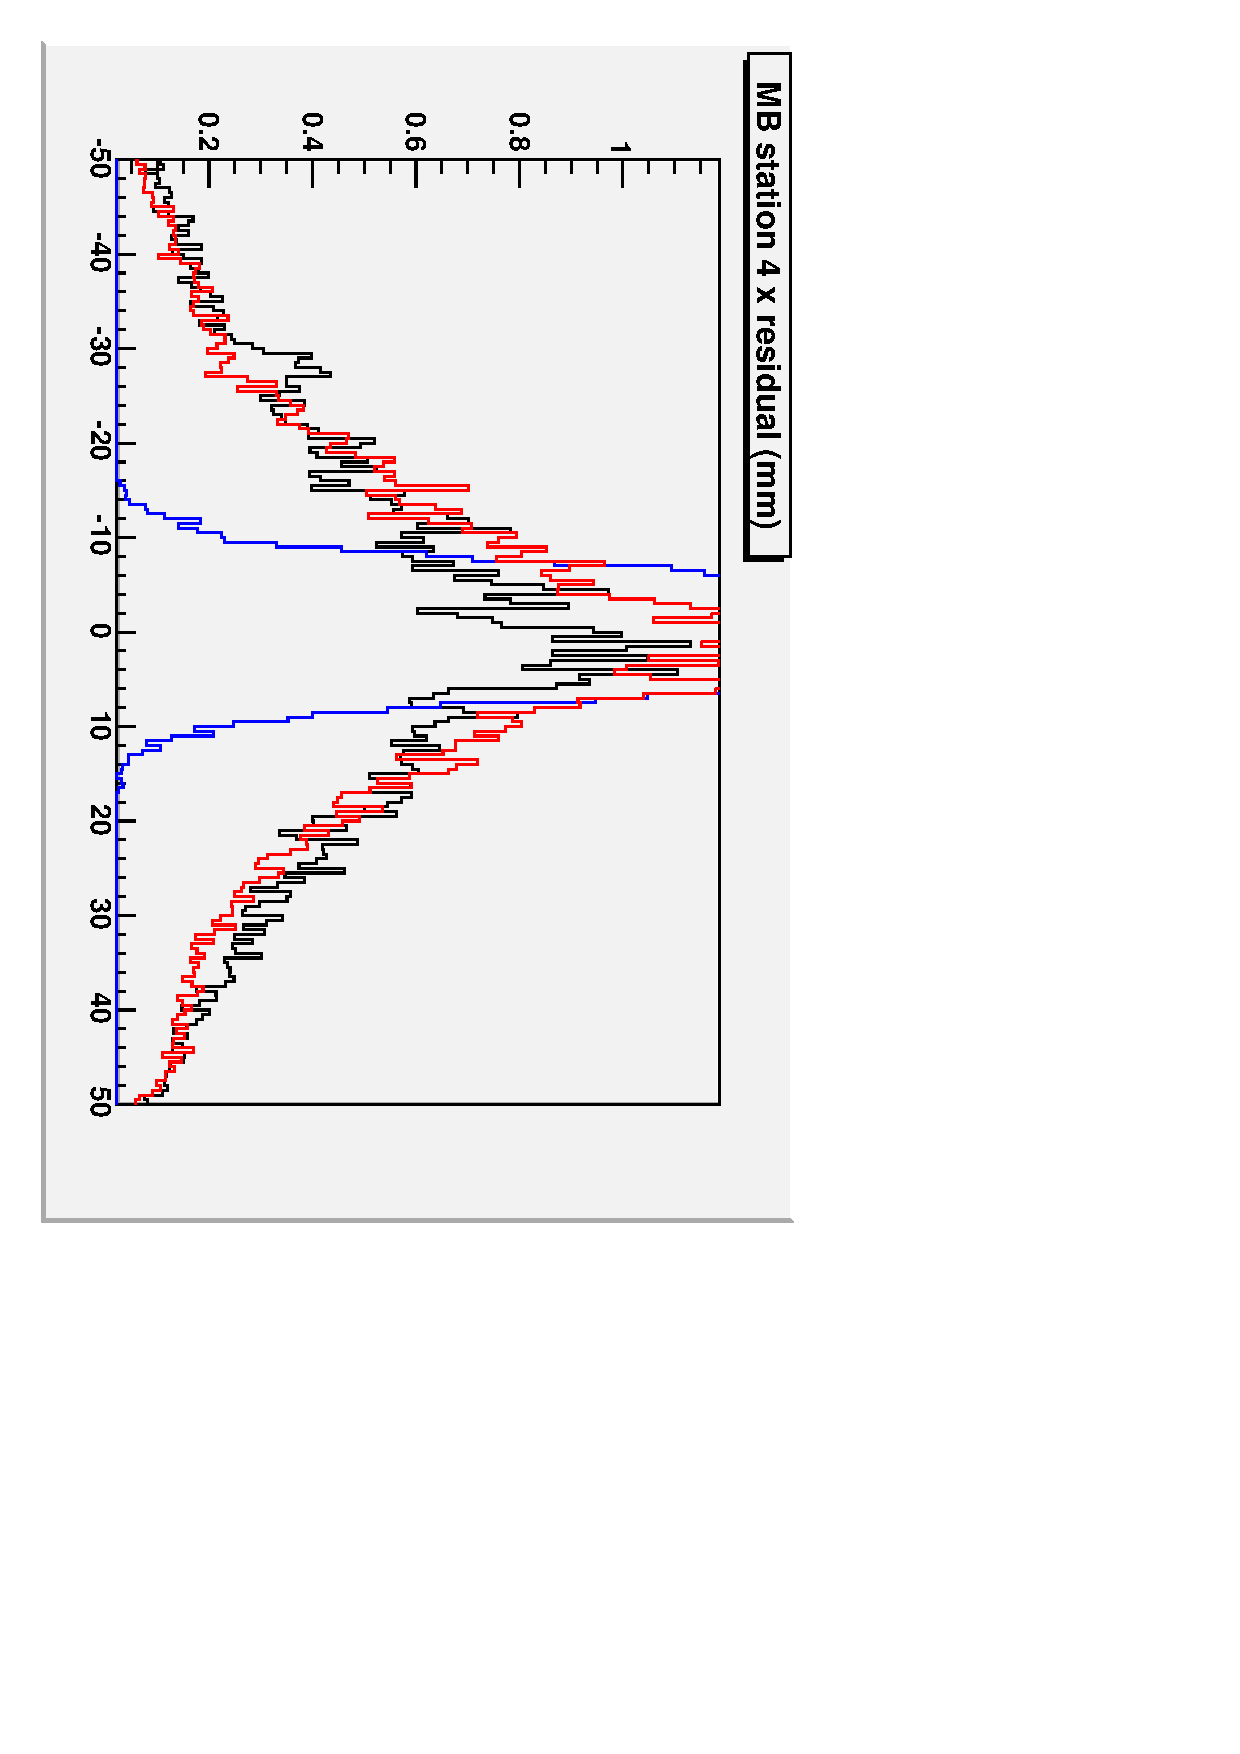
\includegraphics[height=\linewidth, angle=90]{xresid_mb4.pdf}}

\small
Black: FullSim, \textcolor{red}{Red: new FastSim,} \textcolor{blue}{Blue: FastSim without MS}

Local $x$ (global $r\phi$) residuals for tracks propagated from tracker to \only<1>{MB1}\only<2>{MB2}\only<3>{MB3}\only<4>{MB4}
\end{frame}

\begin{frame}
\frametitle{Chamber-by-chamber stdev}
One histogram entry per chamber, one station per plot

\begin{columns}
\column{0.5\linewidth}
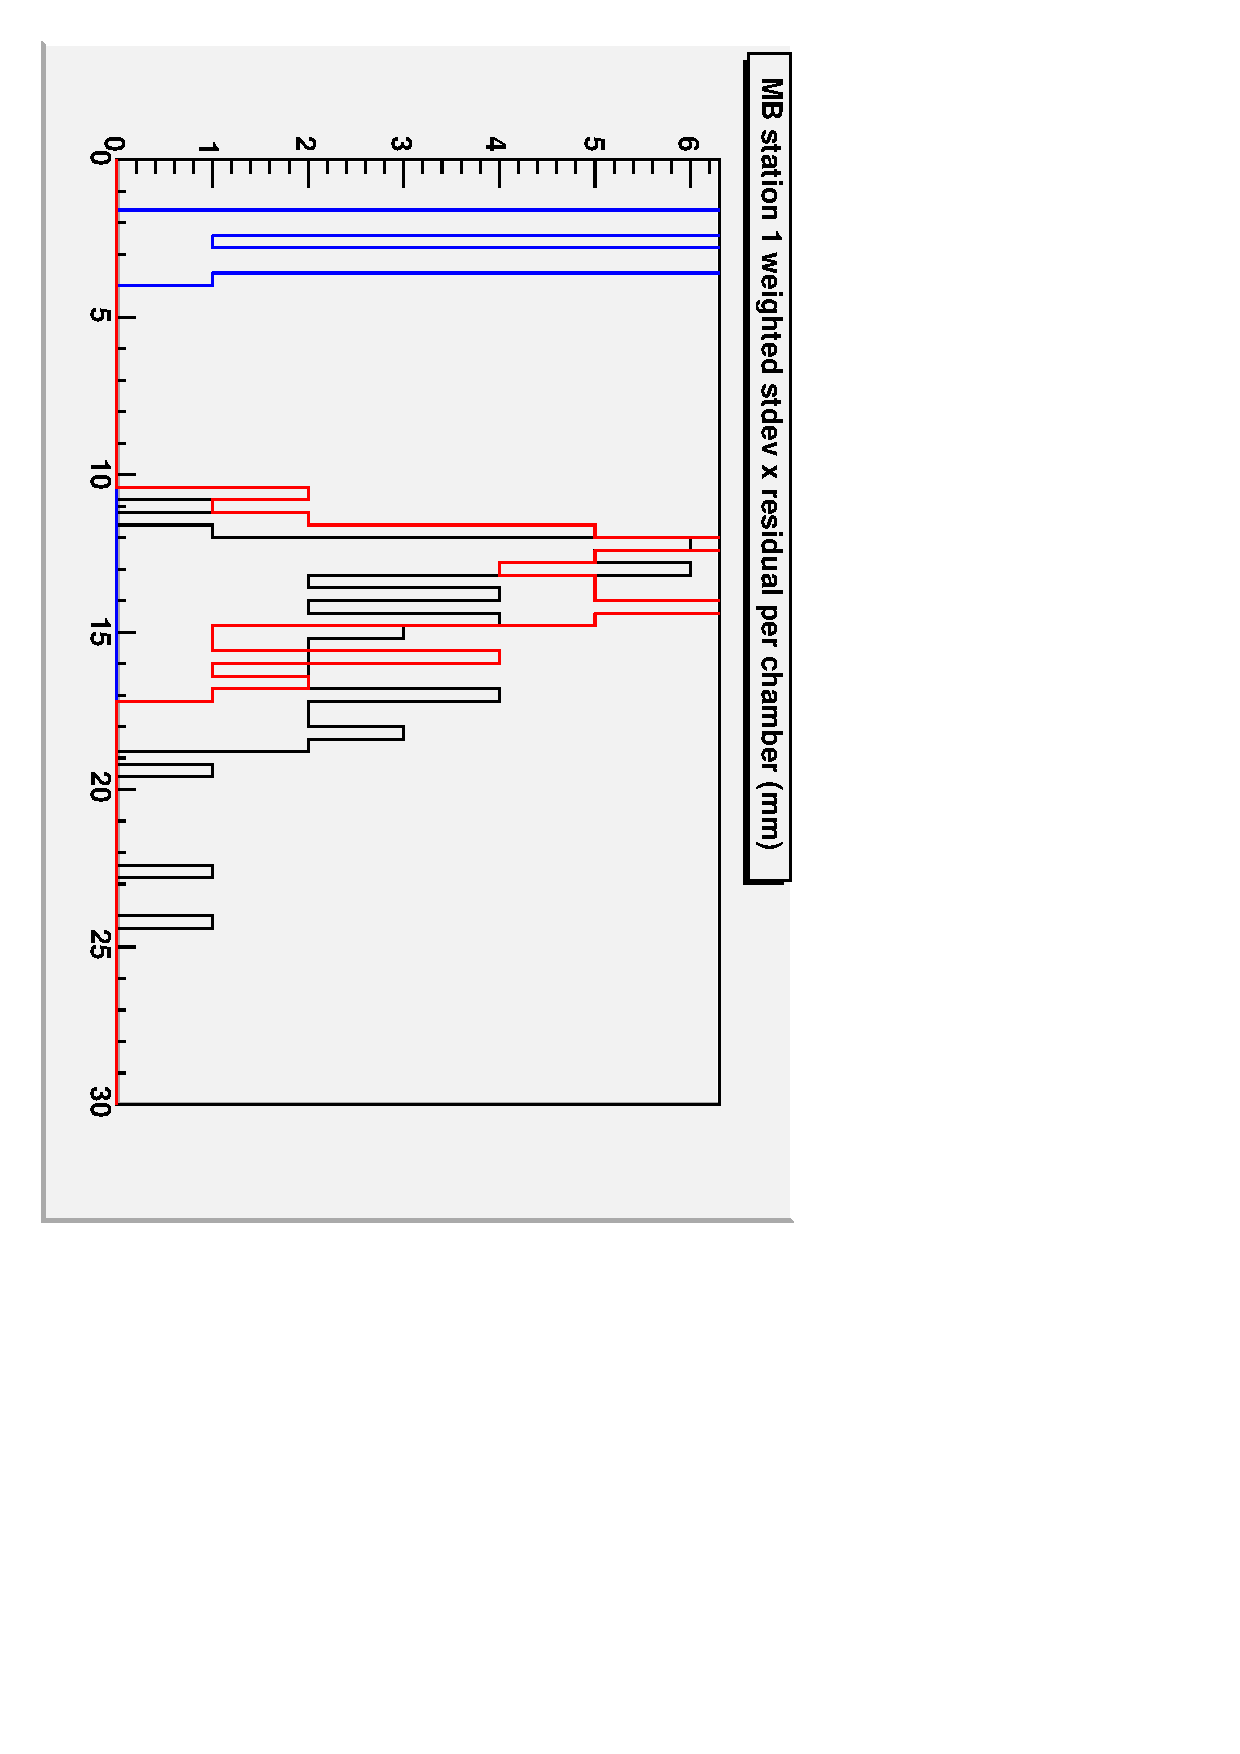
\includegraphics[height=\linewidth, angle=90]{stdevs_mb1.pdf}

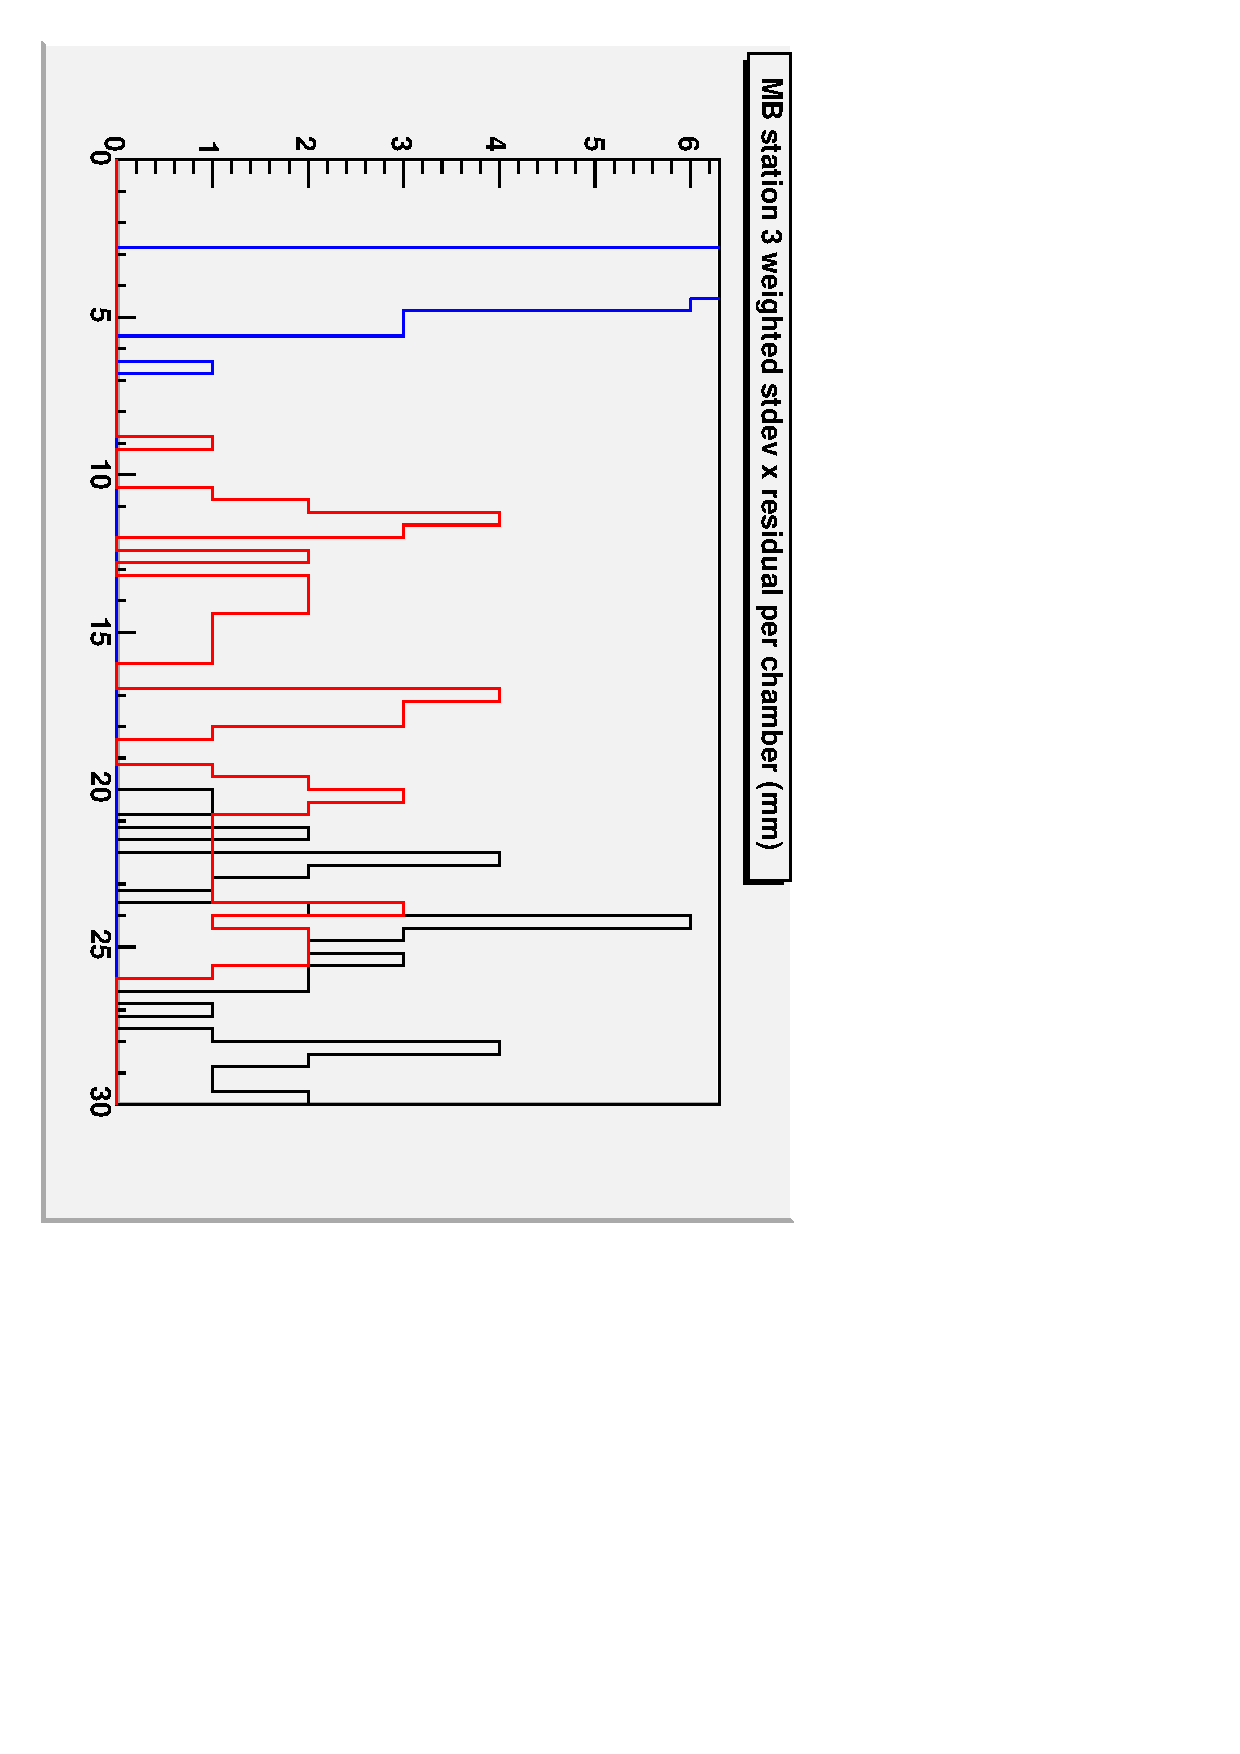
\includegraphics[height=\linewidth, angle=90]{stdevs_mb3.pdf}

\column{0.5\linewidth}
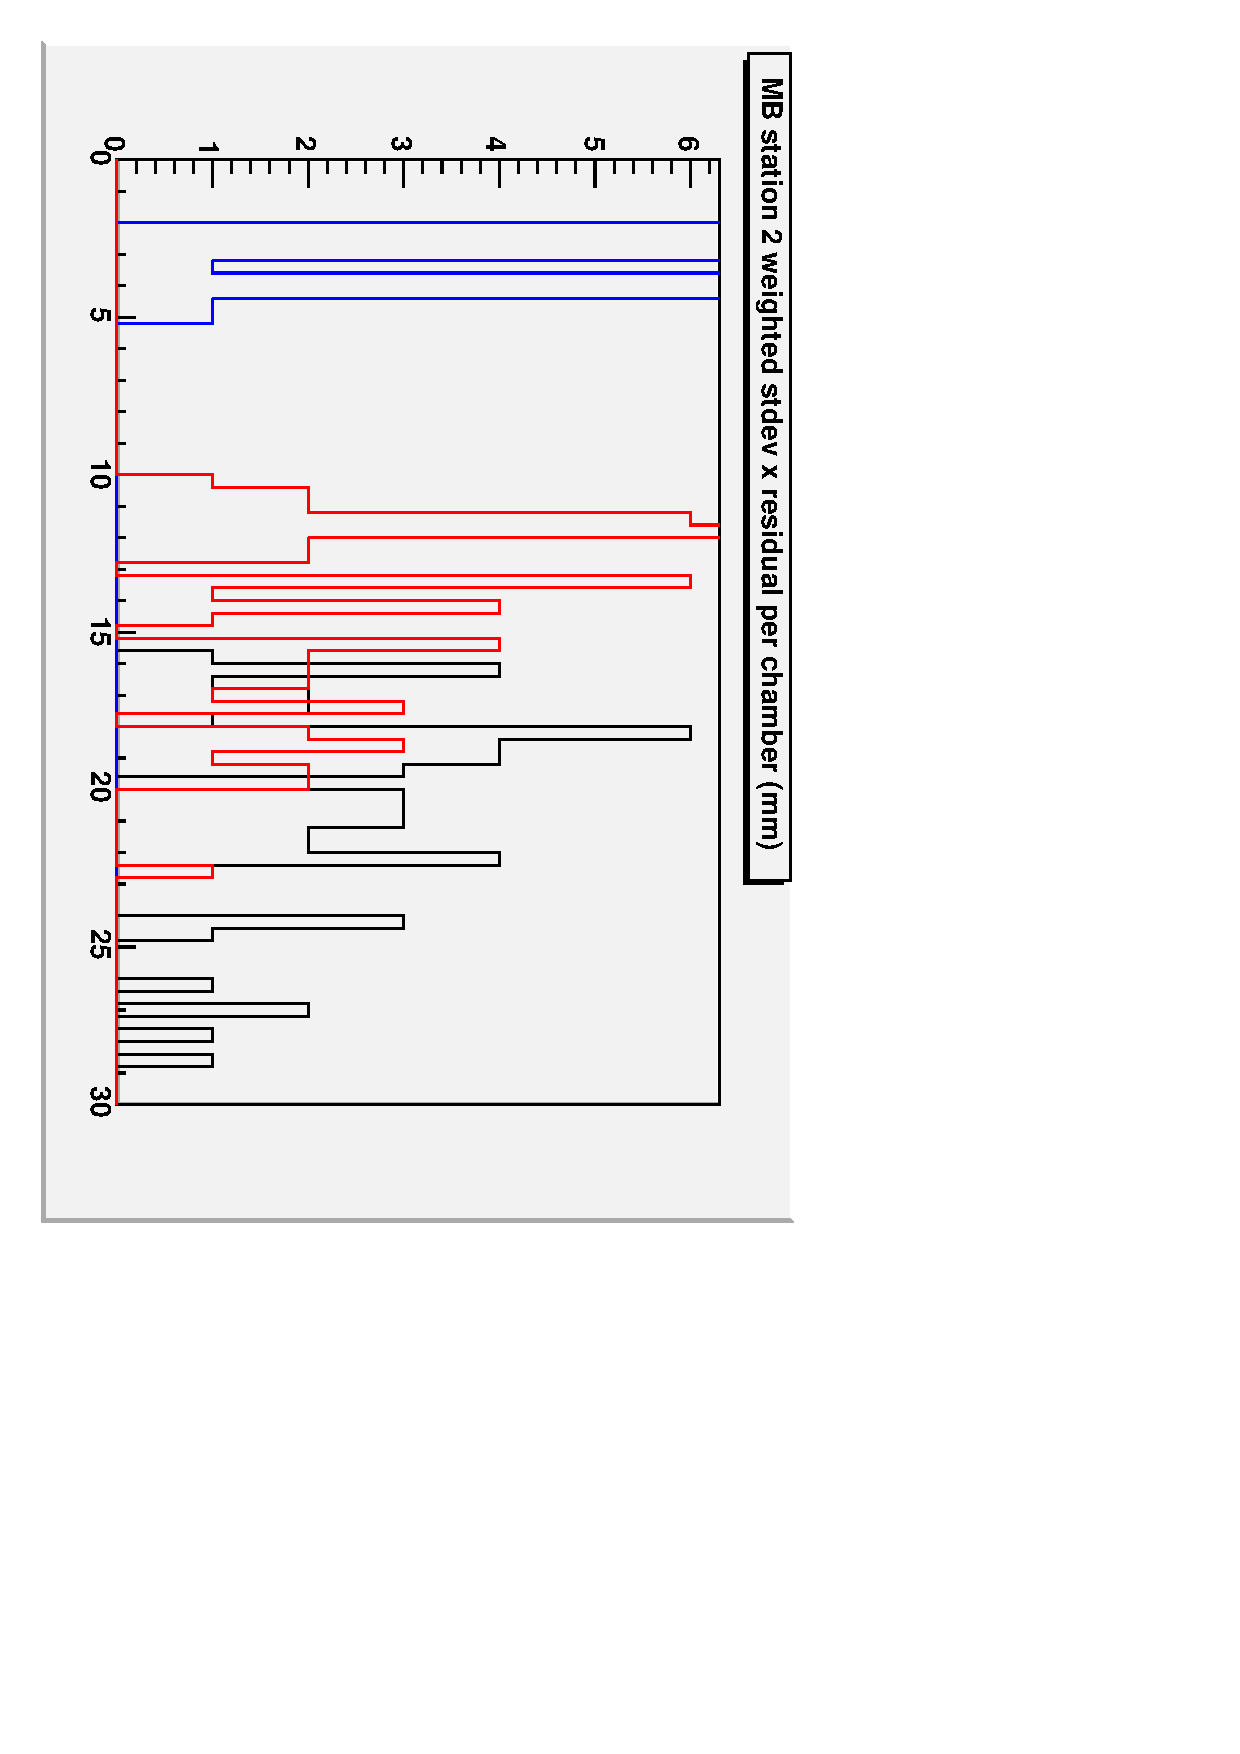
\includegraphics[height=\linewidth, angle=90]{stdevs_mb2.pdf}

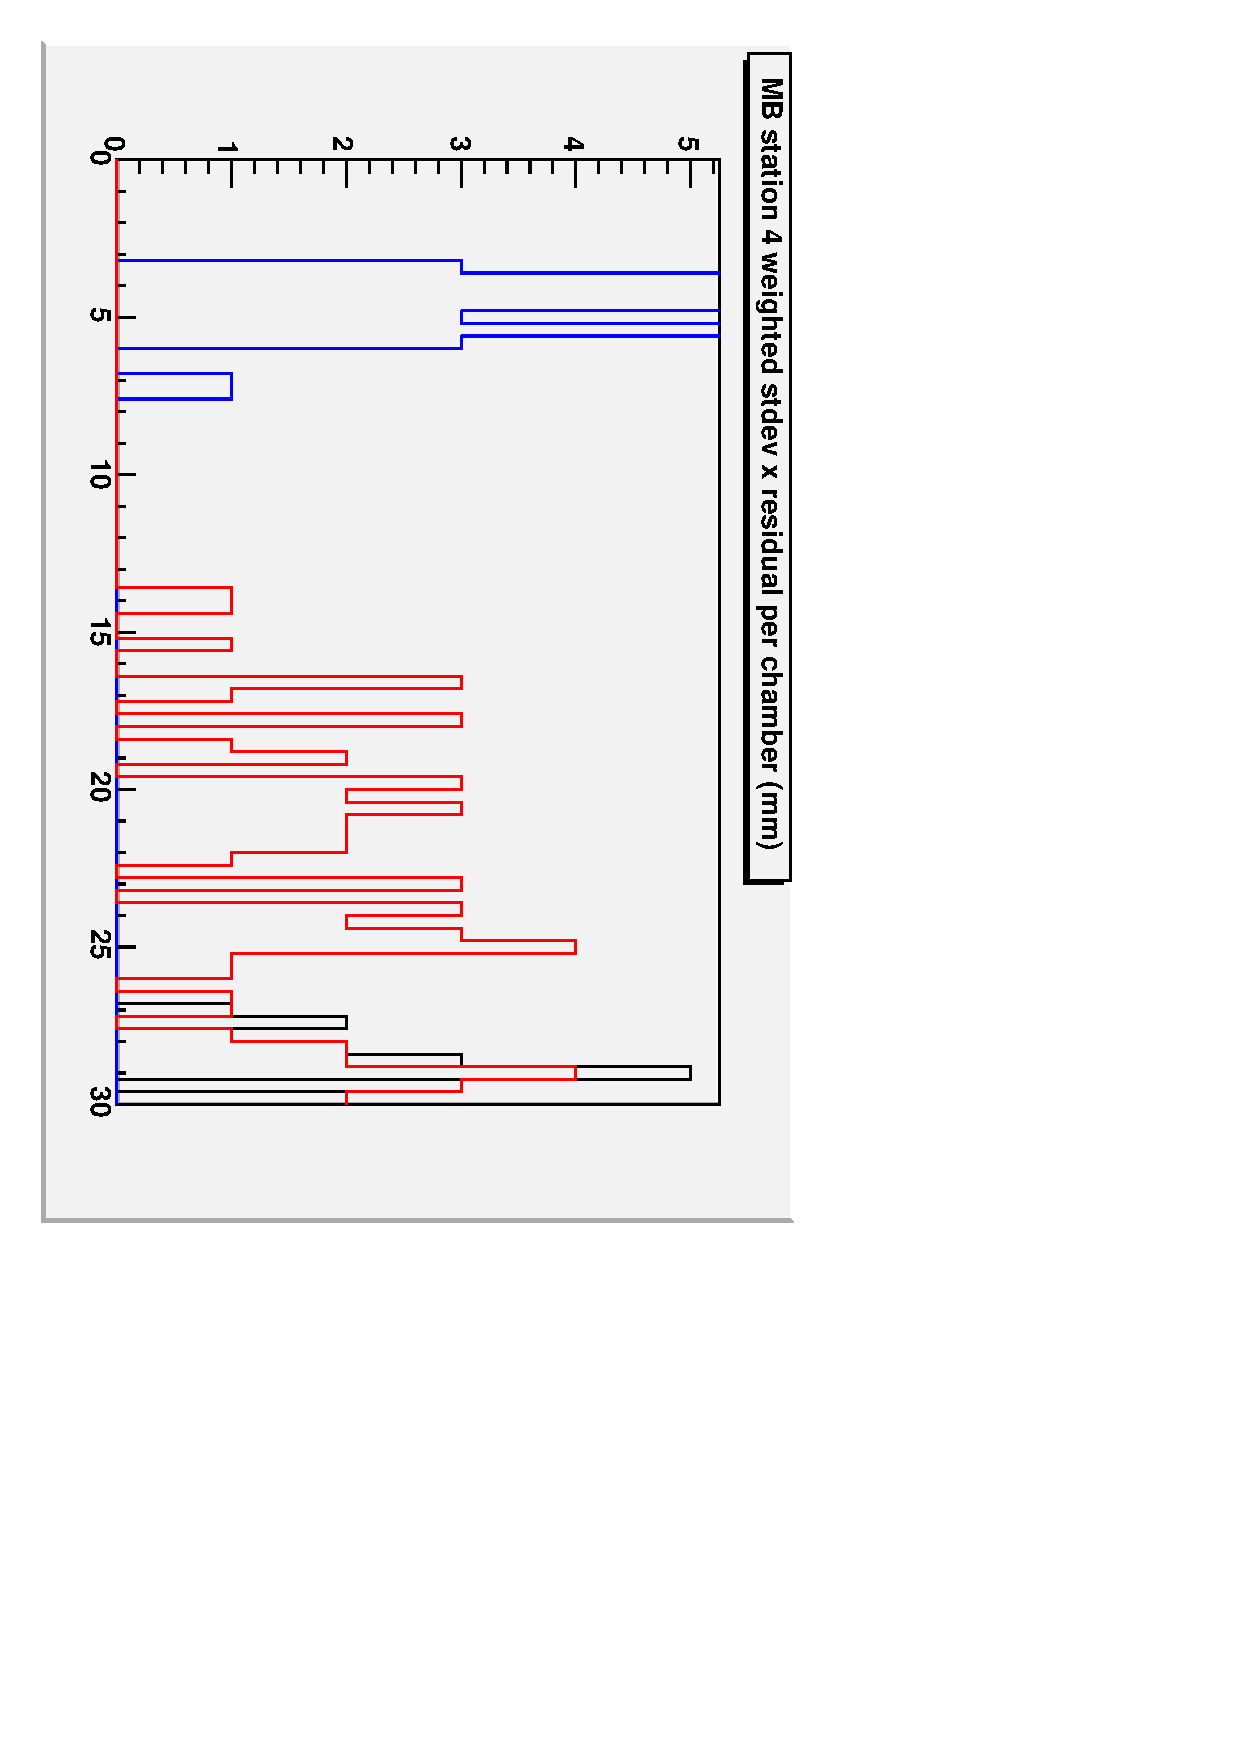
\includegraphics[height=\linewidth, angle=90]{stdevs_mb4.pdf}
\end{columns}

\small
Black: FullSim, \textcolor{red}{Red: new FastSim,} \textcolor{blue}{Blue: FastSim without MS}
\end{frame}

\begin{frame}
\frametitle{Endcap station 1}
One histogram entry per chamber, one station per plot

\begin{columns}
\column{0.5\linewidth}
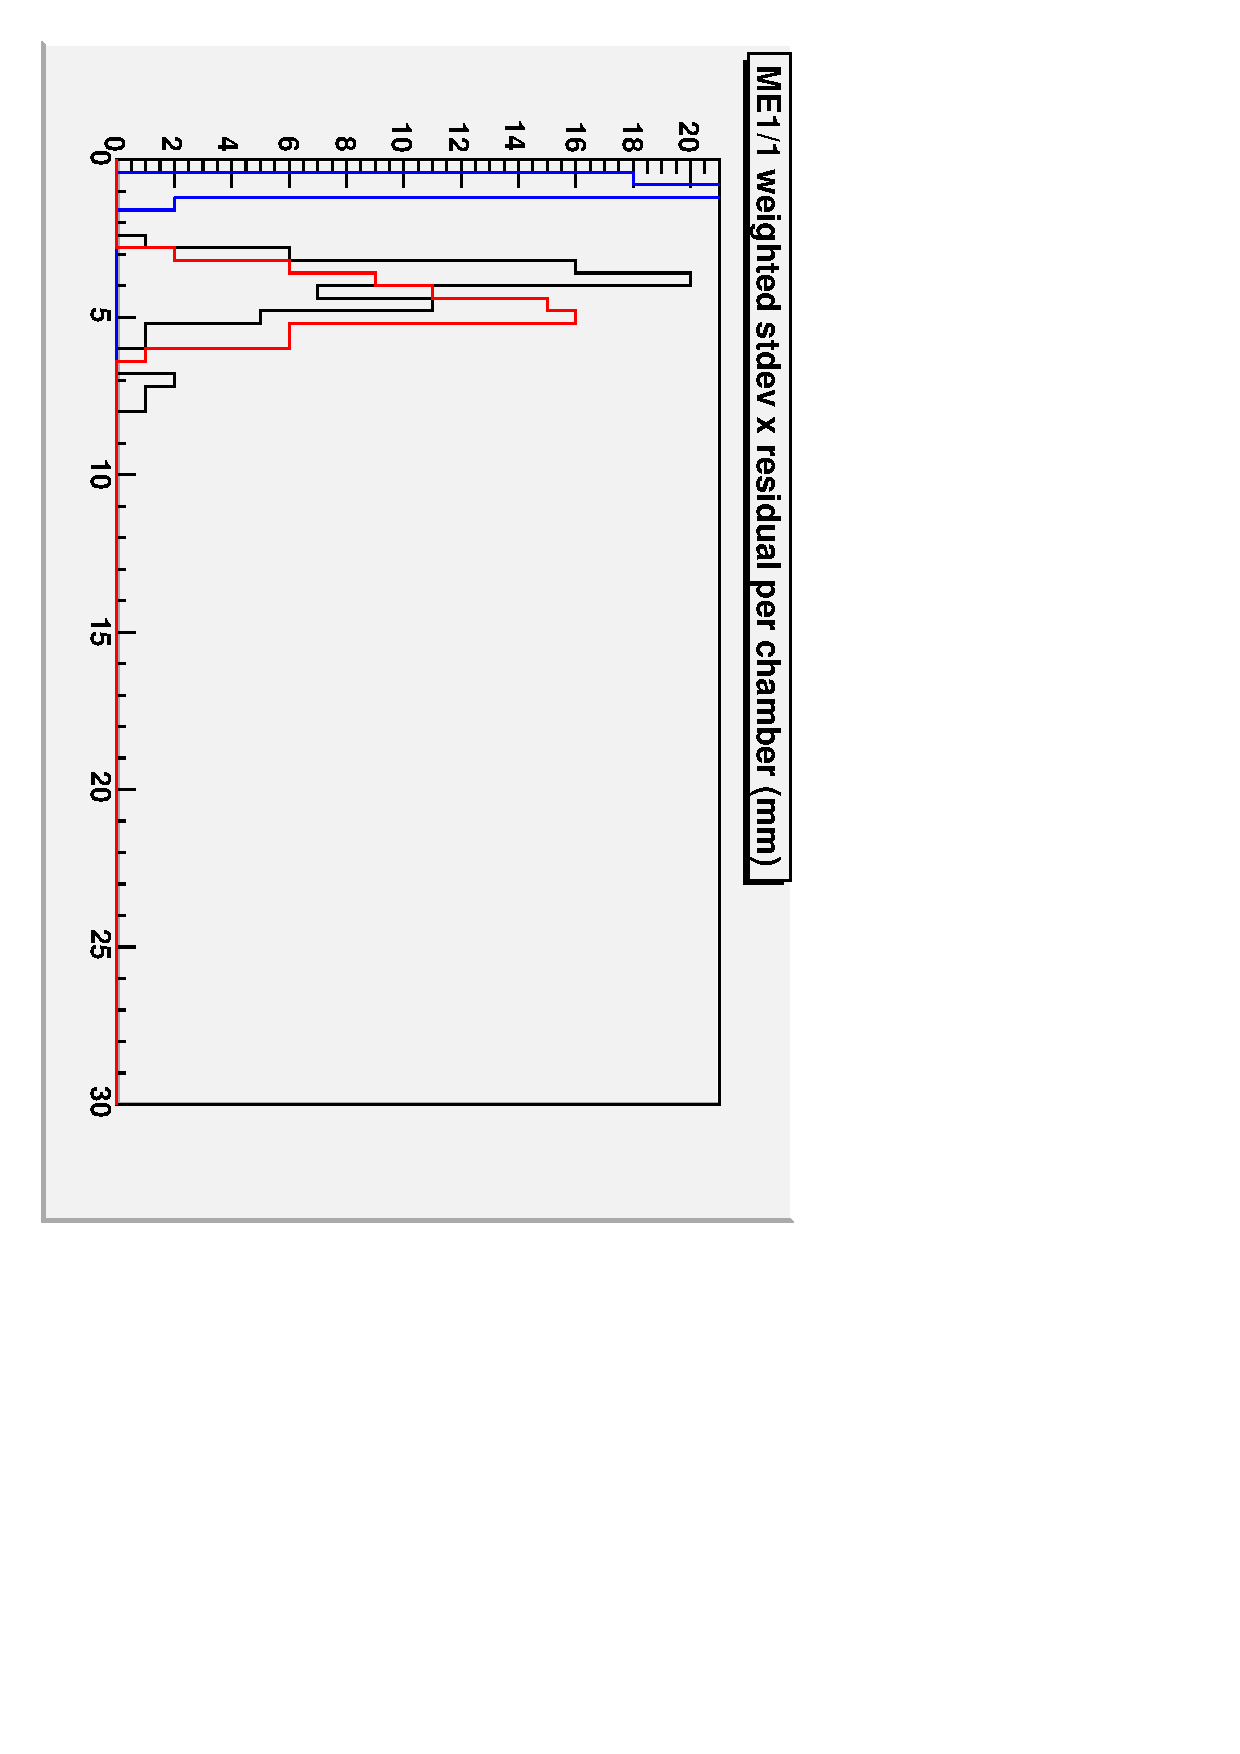
\includegraphics[height=\linewidth, angle=90]{stdevs_me11.pdf}

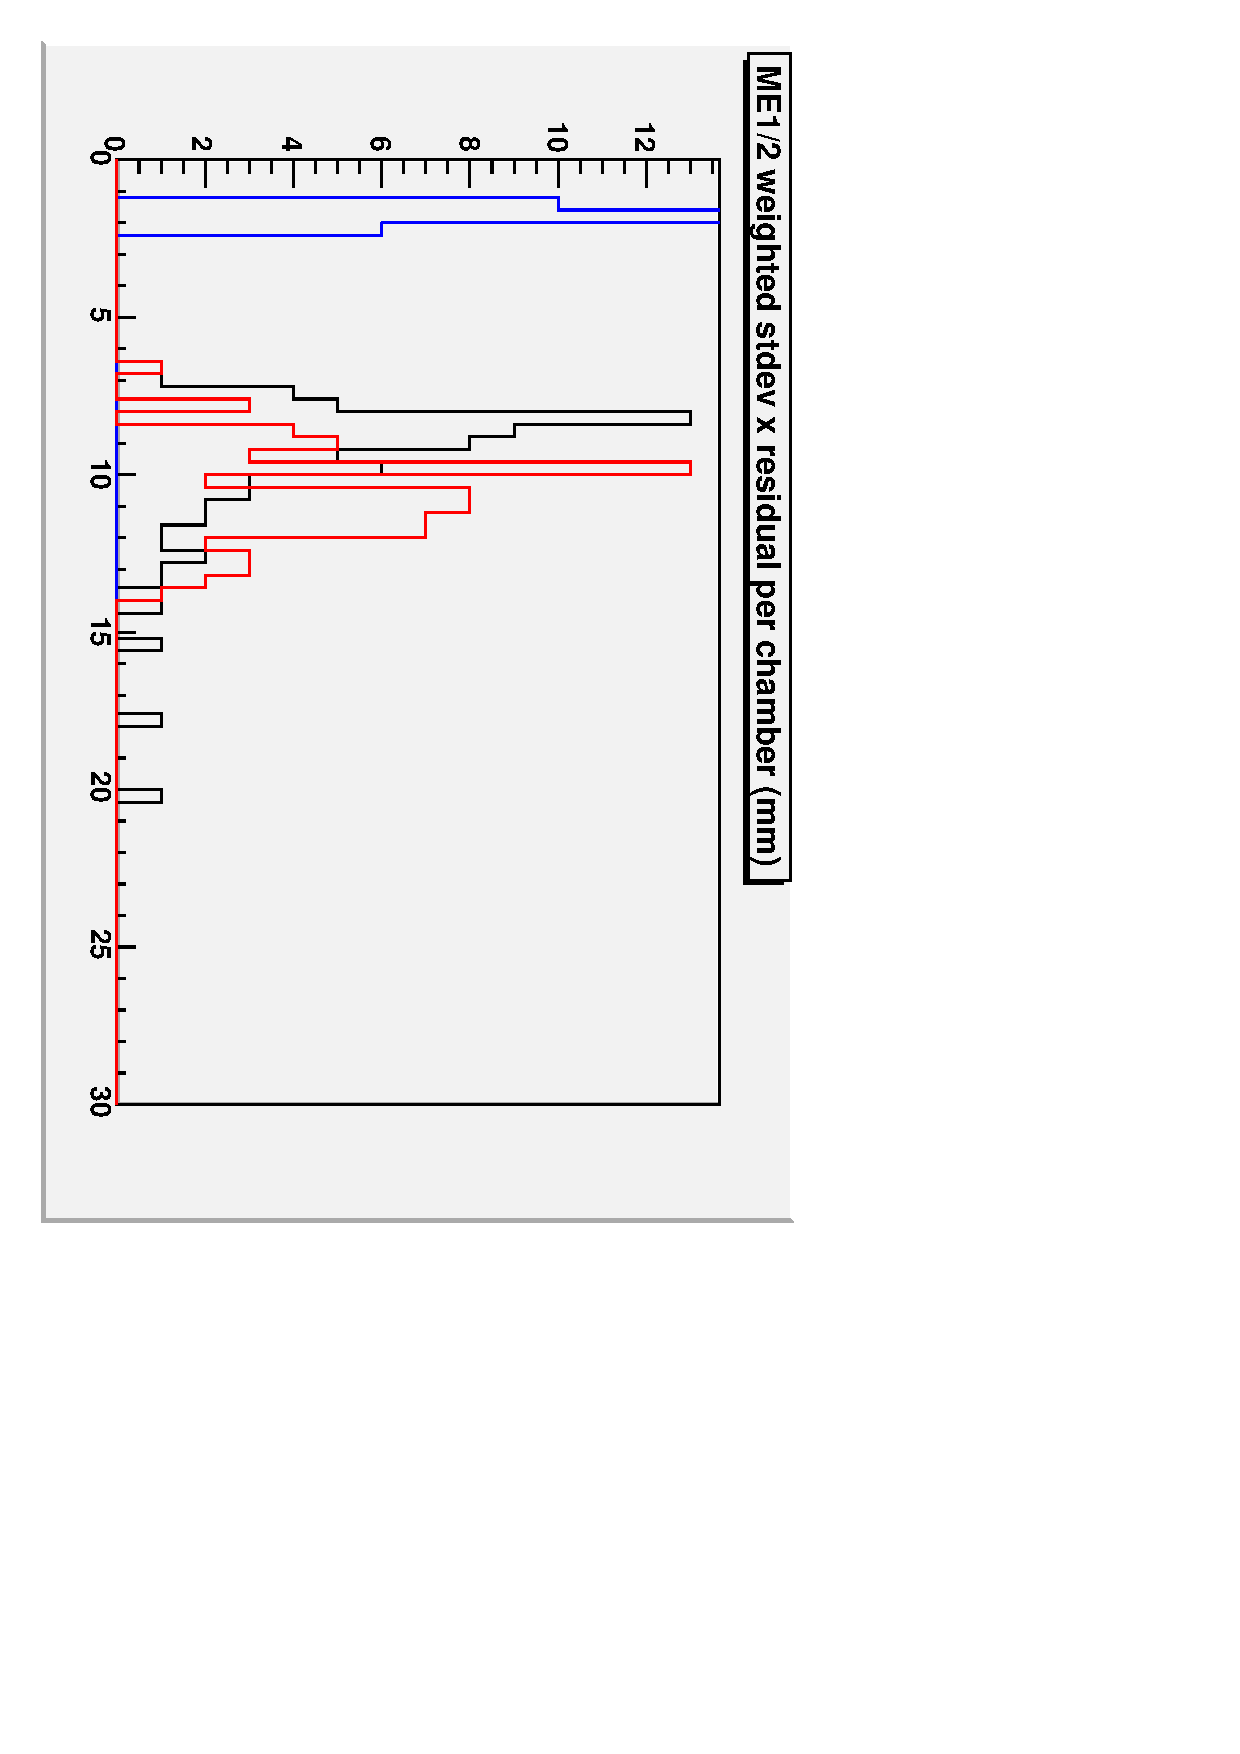
\includegraphics[height=\linewidth, angle=90]{stdevs_me12.pdf}

\column{0.5\linewidth}
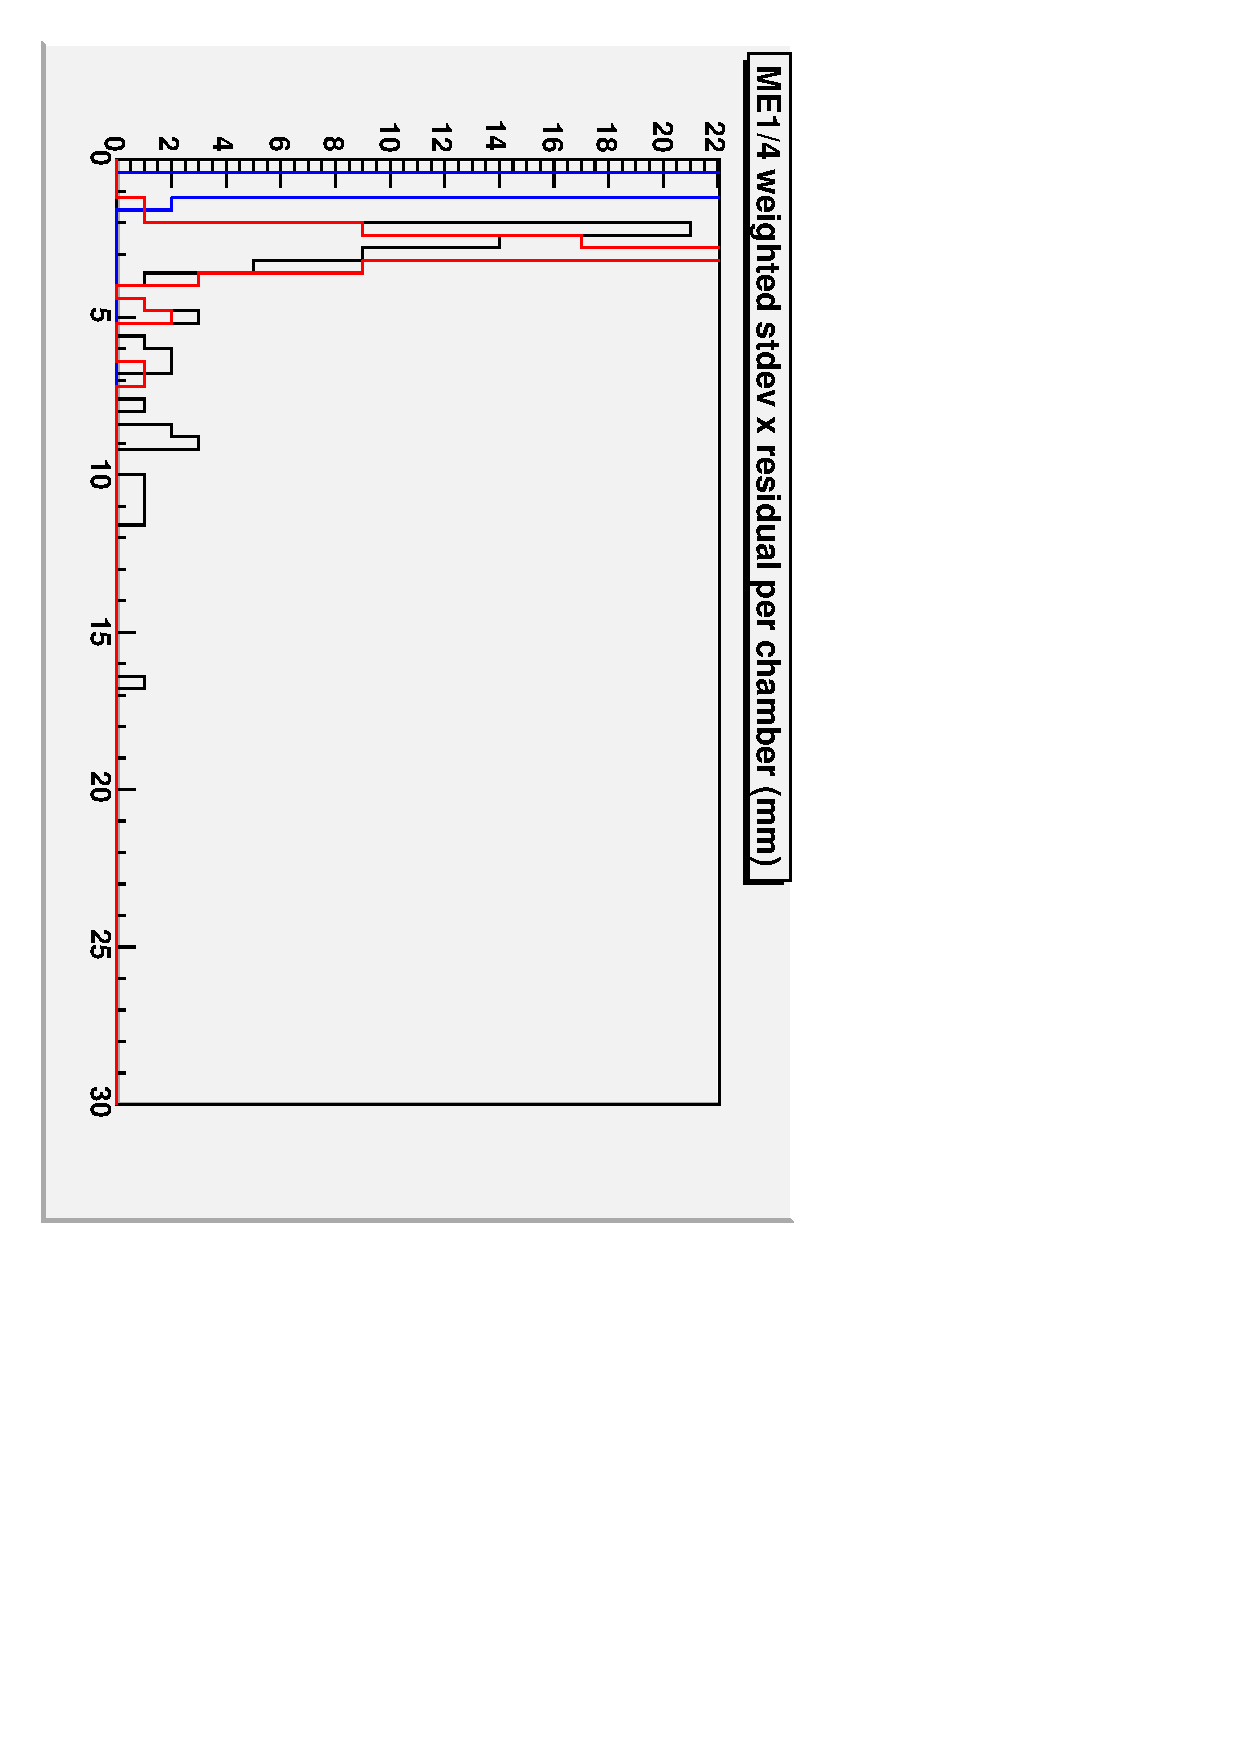
\includegraphics[height=\linewidth, angle=90]{stdevs_me14.pdf}

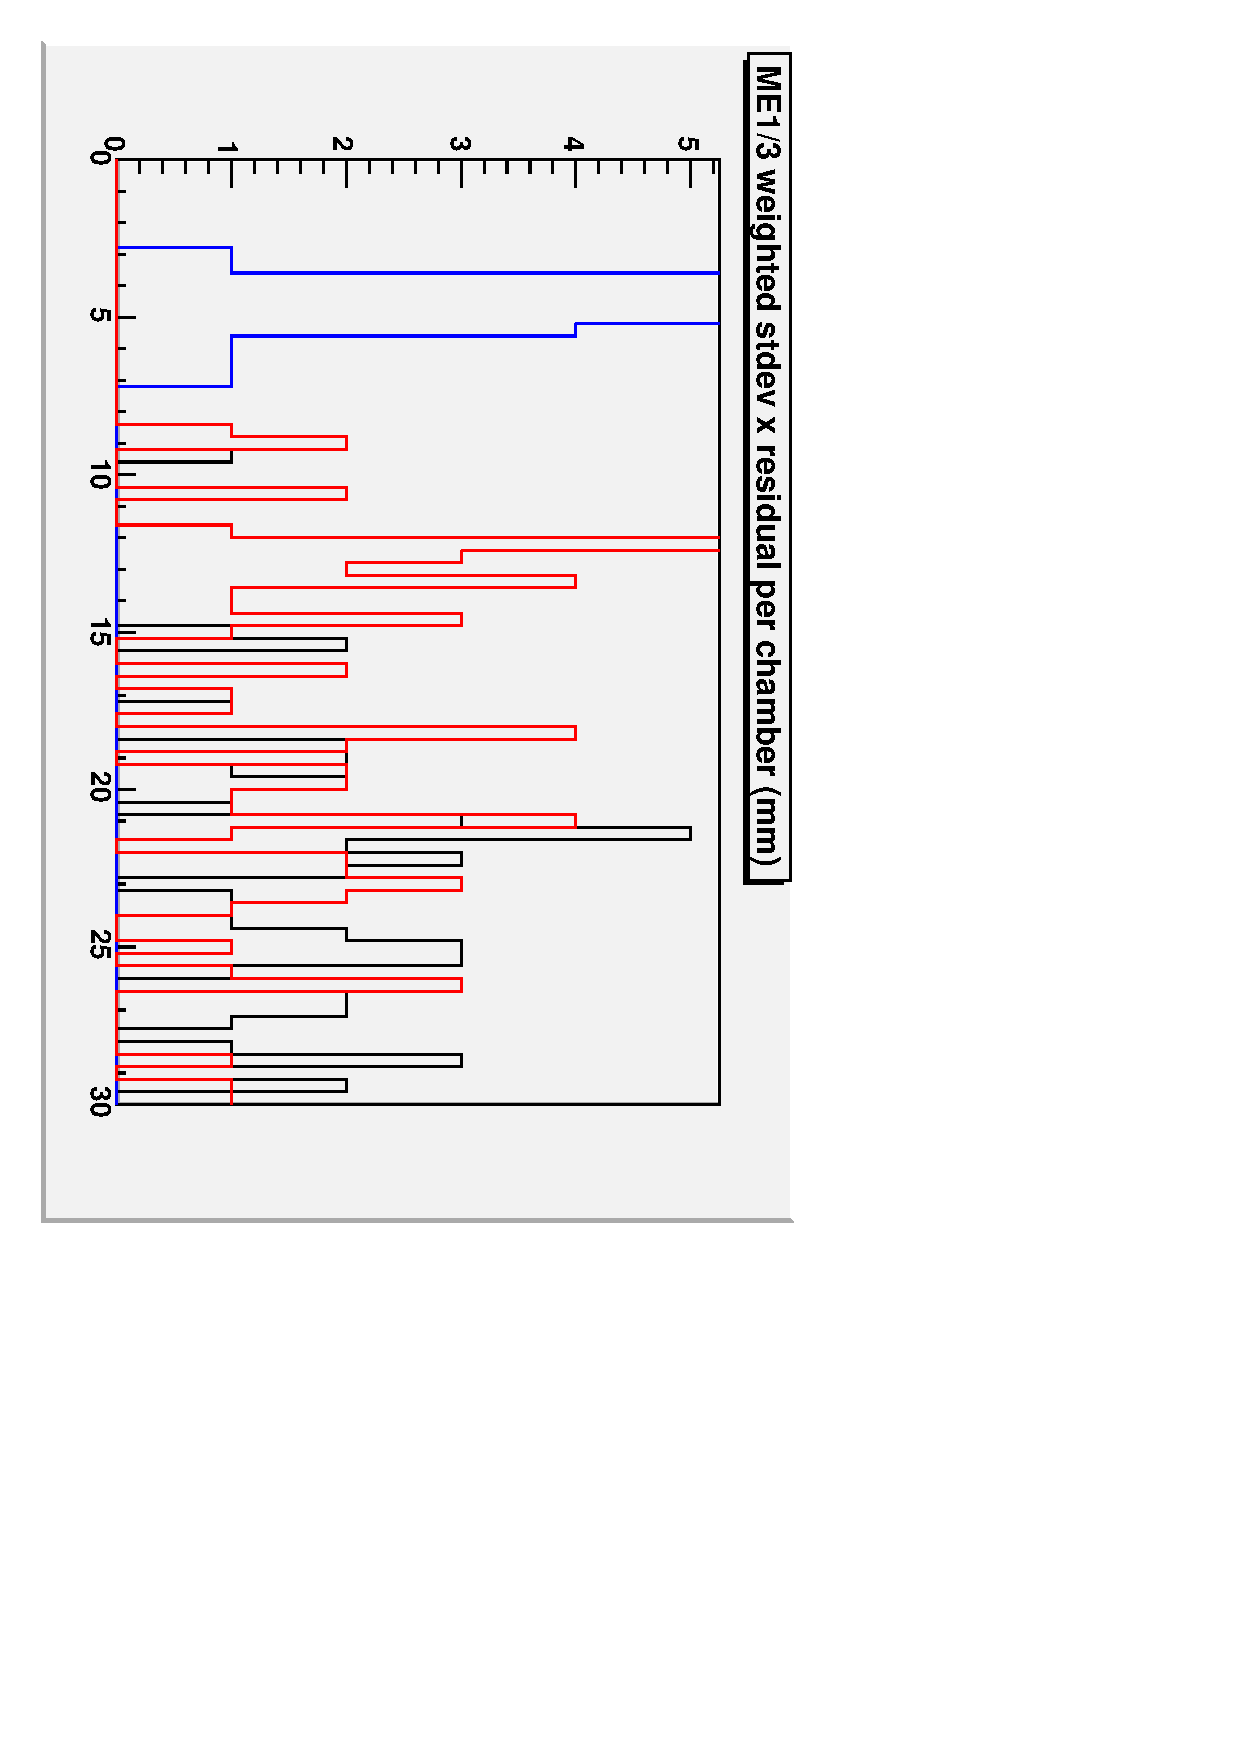
\includegraphics[height=\linewidth, angle=90]{stdevs_me13.pdf}
\end{columns}

\small
Black: FullSim, \textcolor{red}{Red: new FastSim,} \textcolor{blue}{Blue: FastSim without MS}
\end{frame}

\begin{frame}
\frametitle{Endcap station 2 and 3}
One histogram entry per chamber, one station per plot

\begin{columns}
\column{0.5\linewidth}
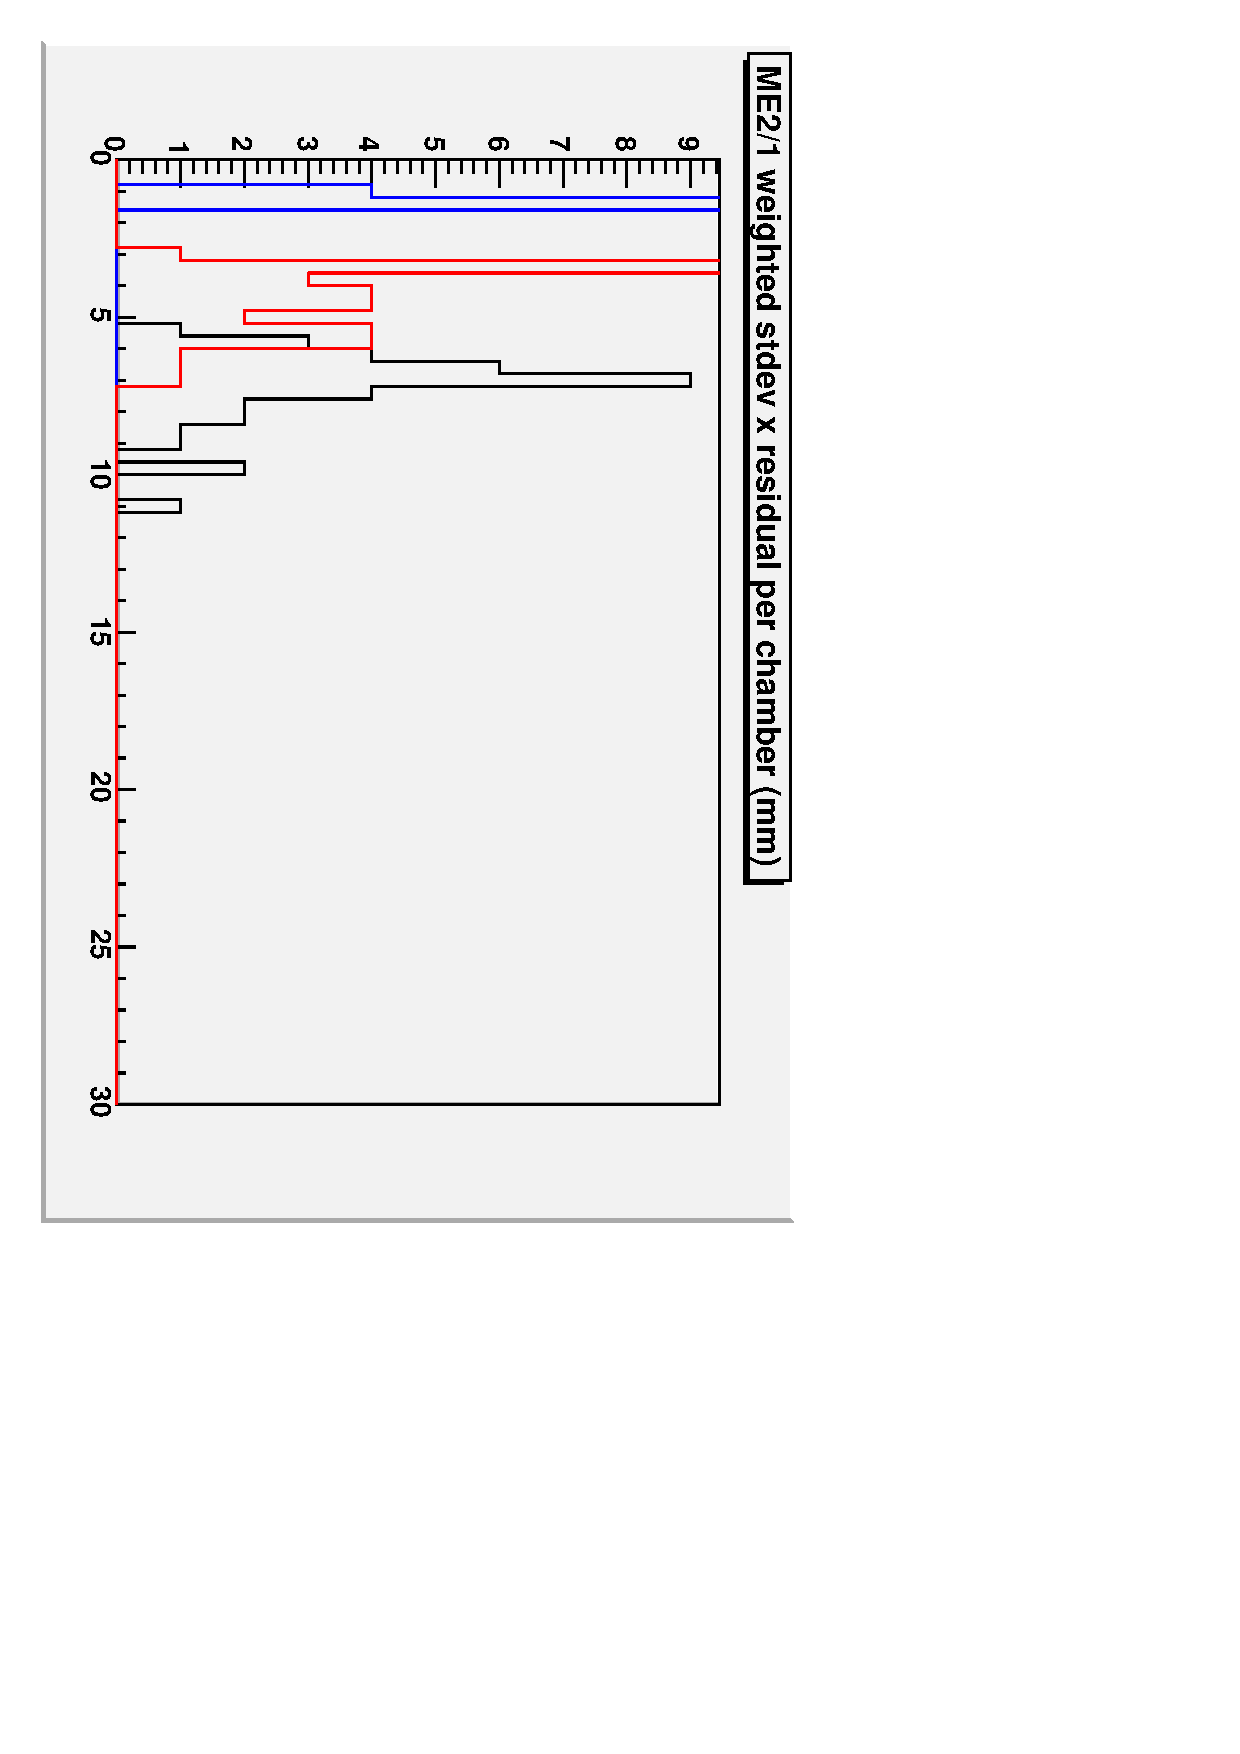
\includegraphics[height=\linewidth, angle=90]{stdevs_me21.pdf}

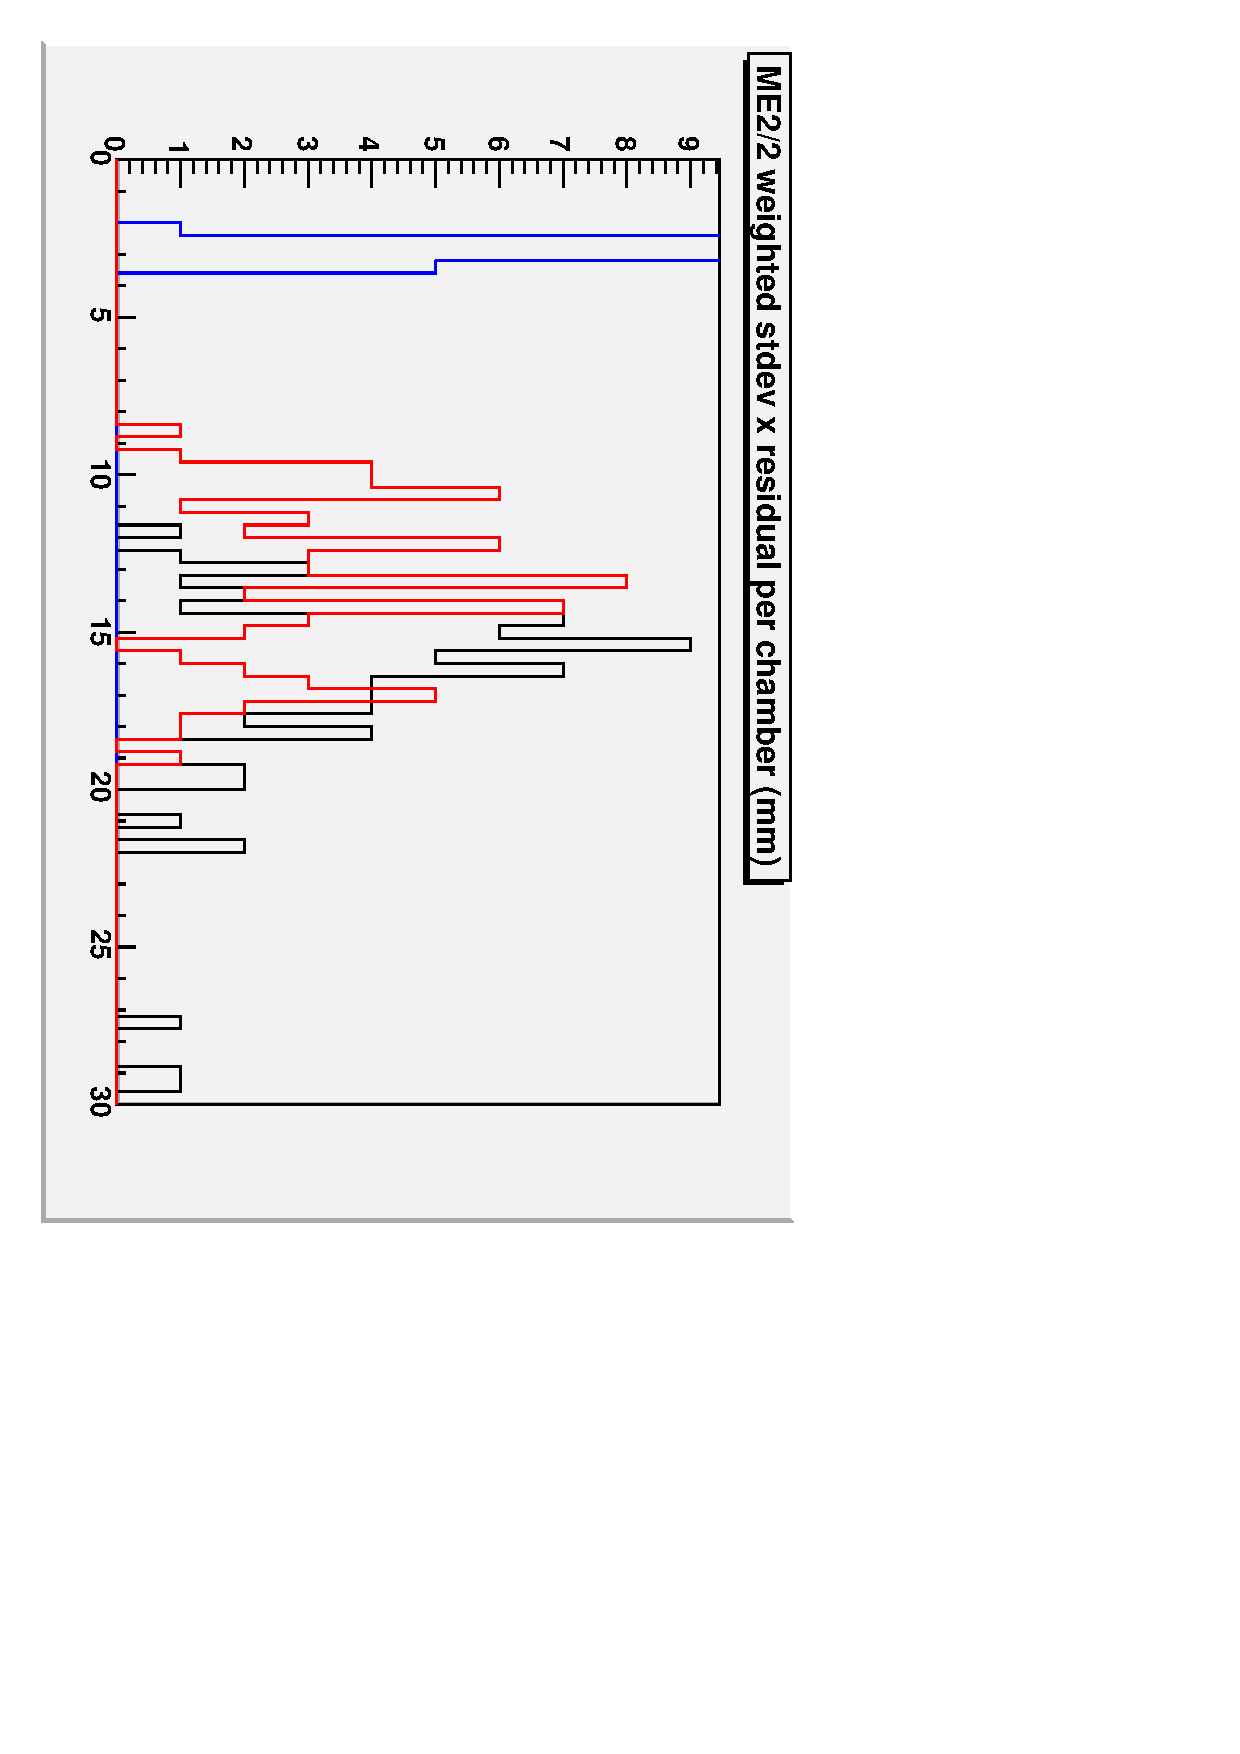
\includegraphics[height=\linewidth, angle=90]{stdevs_me22.pdf}

\column{0.5\linewidth}
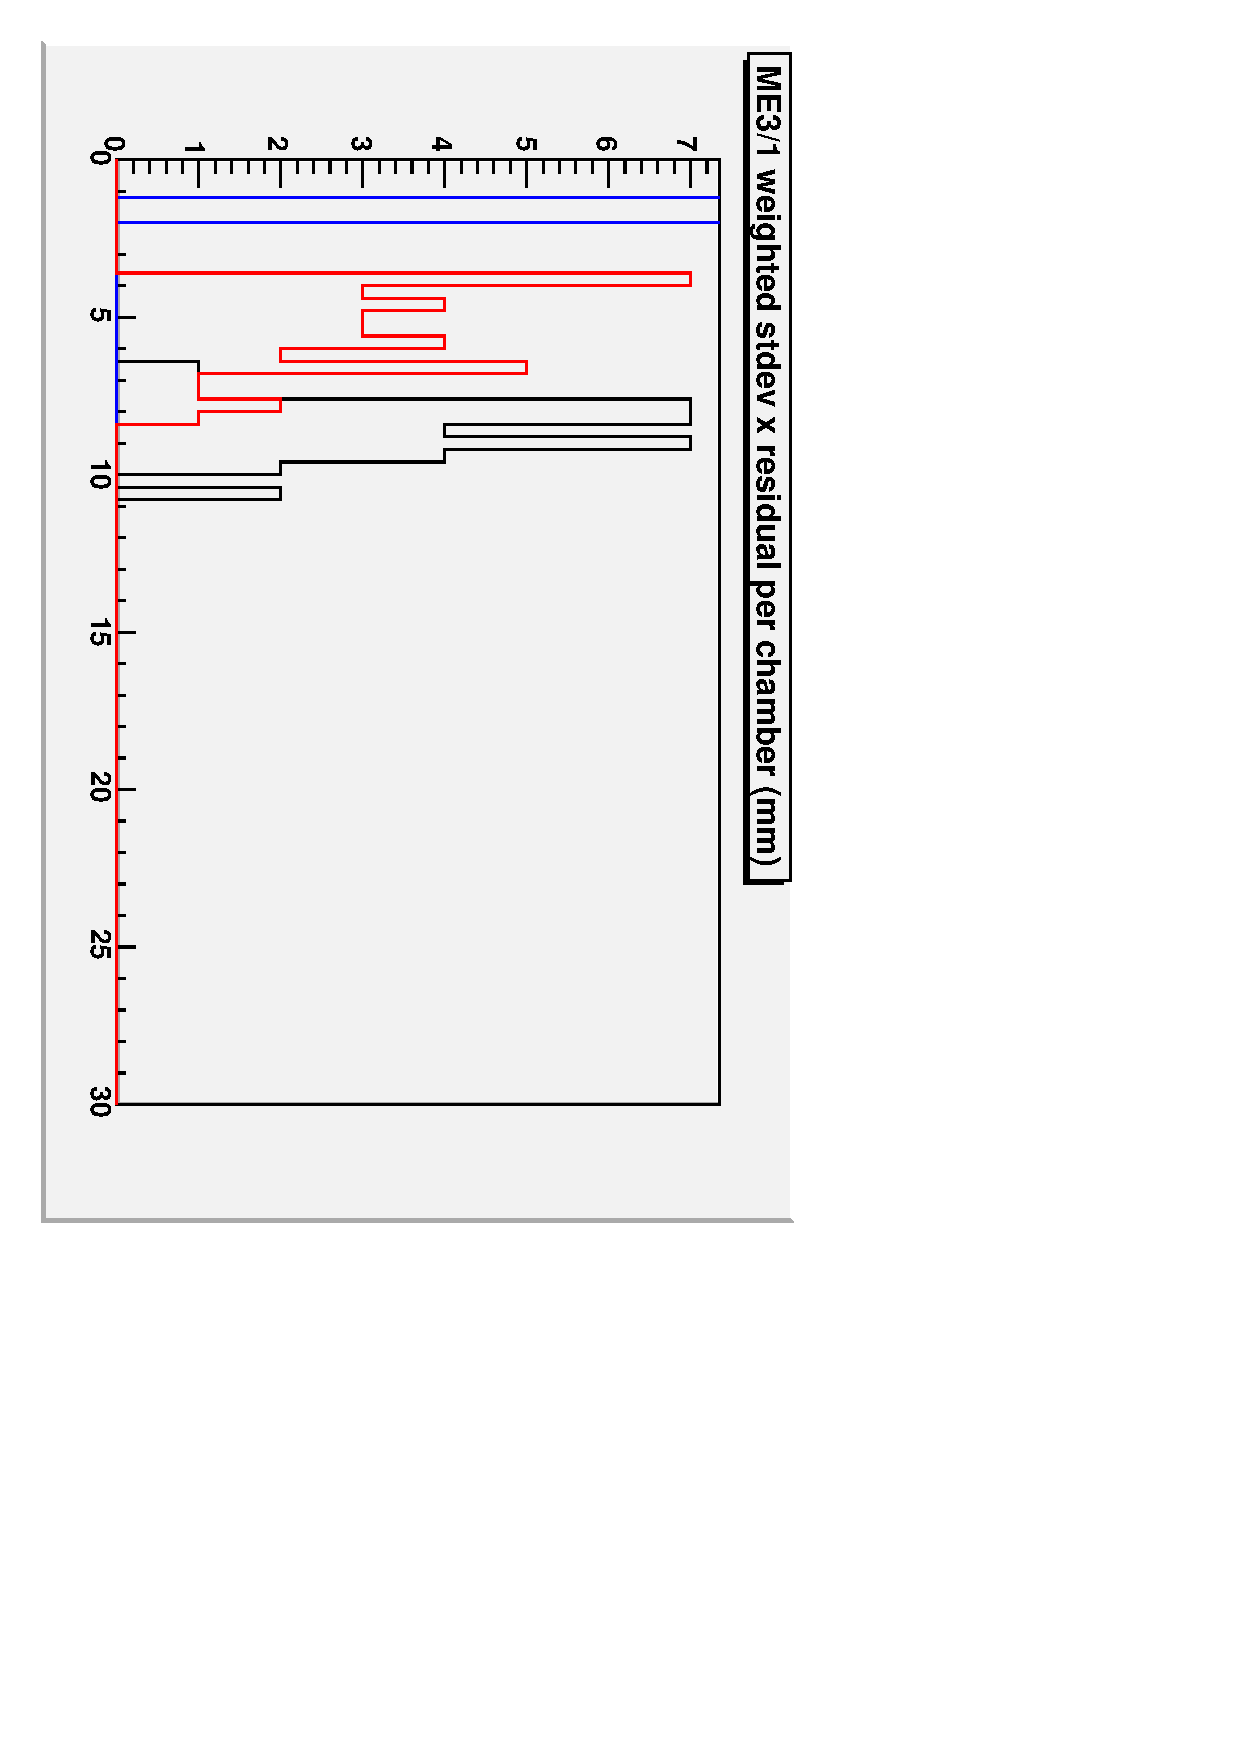
\includegraphics[height=\linewidth, angle=90]{stdevs_me31.pdf}

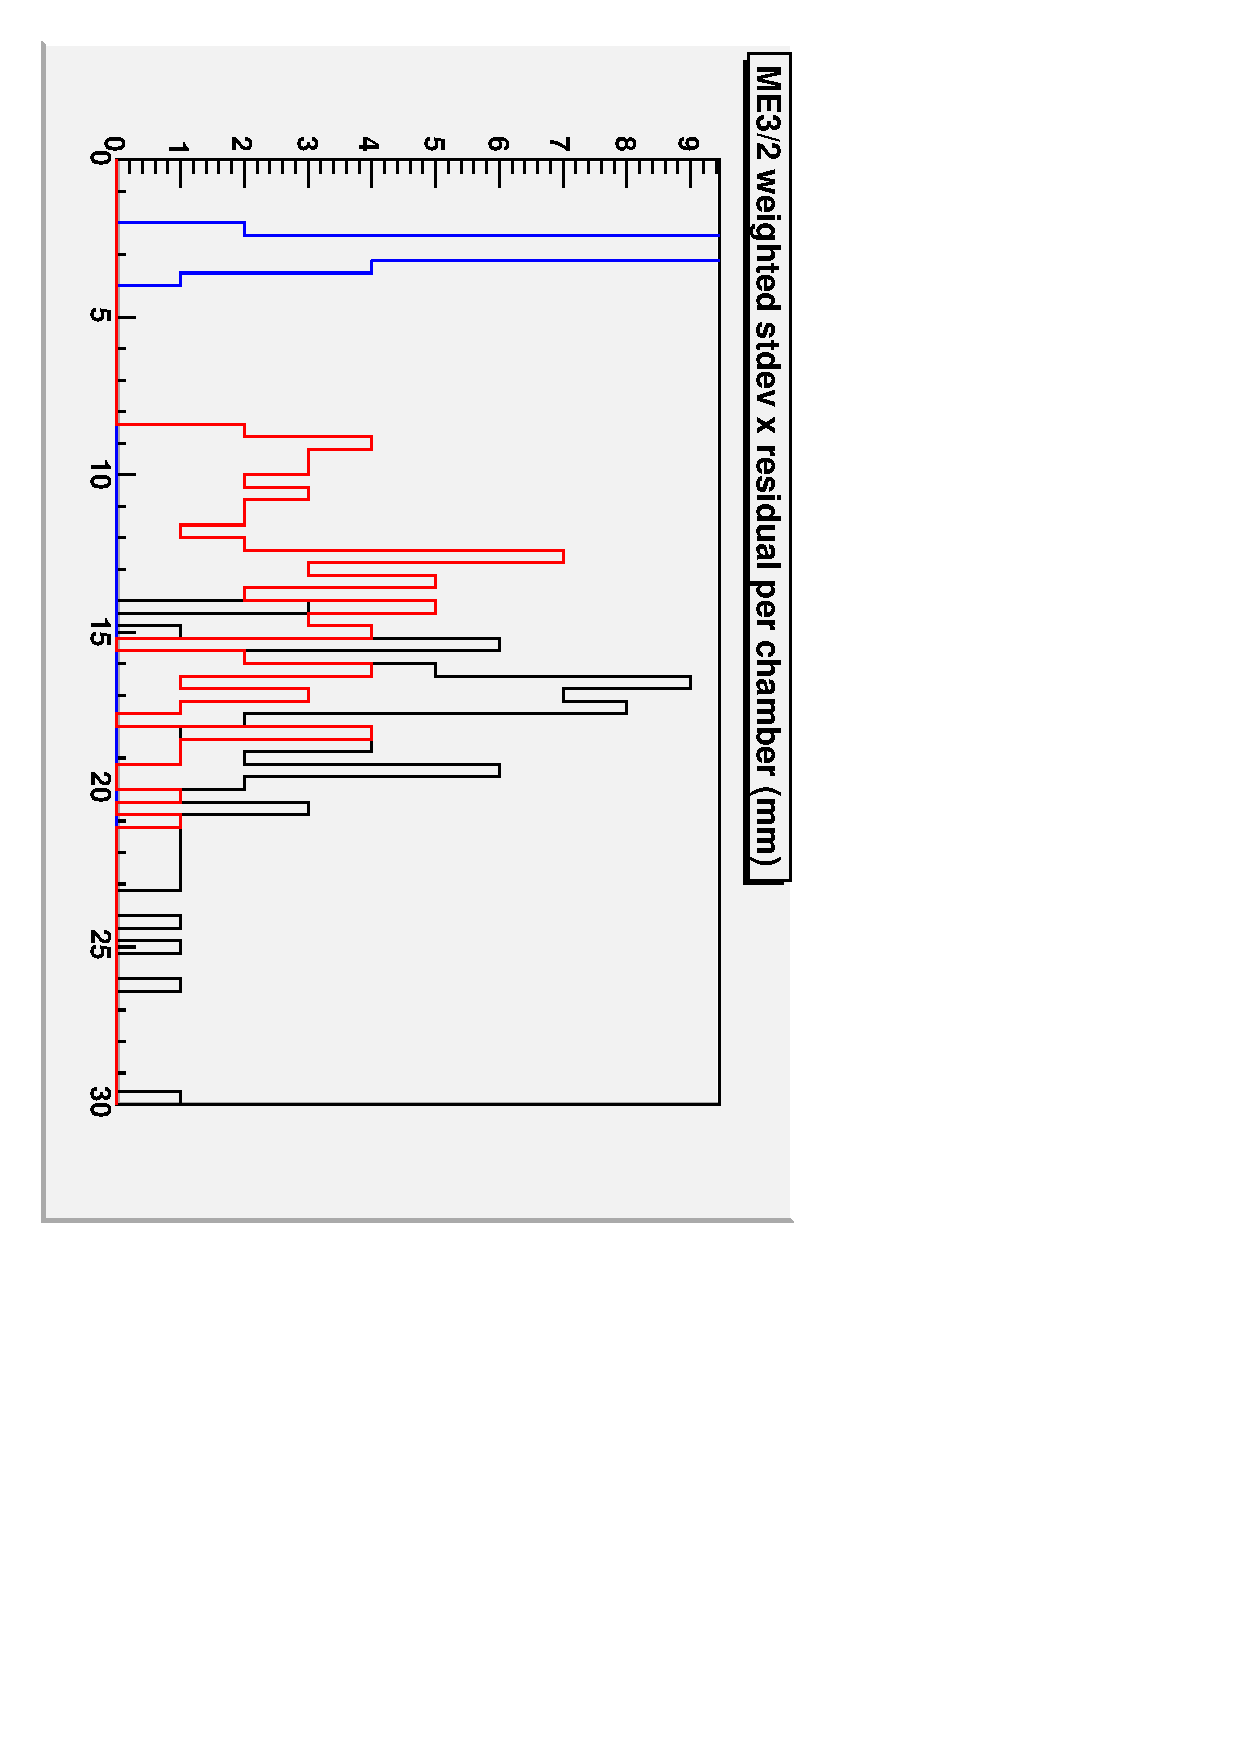
\includegraphics[height=\linewidth, angle=90]{stdevs_me32.pdf}
\end{columns}

\small
Black: FullSim, \textcolor{red}{Red: new FastSim,} \textcolor{blue}{Blue: FastSim without MS}
\end{frame}

%% \section*{First section}
%% \begin{frame}
%% \begin{center}
%% \Huge \textcolor{blue}{First section}
%% \end{center}
%% \end{frame}

\begin{frame}
\frametitle{Conclusions}

\begin{itemize}\setlength{\itemsep}{0.2 cm}
\item \textcolor{red}{First implementation of multiple scattering in FastSim}

is a big improvement over \textcolor{blue}{1\_8\_4!}
\item Still underestimated in outer barrel
\item Slightly underestimated in ME1/1 and ME1/2, slightly overestimated in some other endcap stations
\end{itemize}

\begin{columns}
\column{0.5\linewidth}
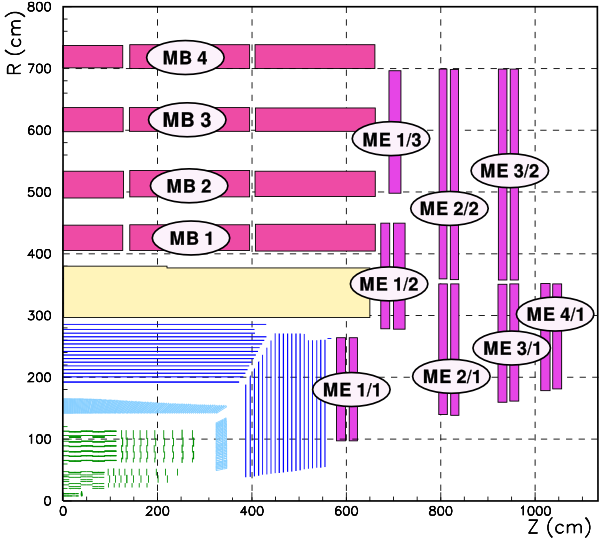
\includegraphics[width=\linewidth]{muon_system.png}

\column{0.5\linewidth}
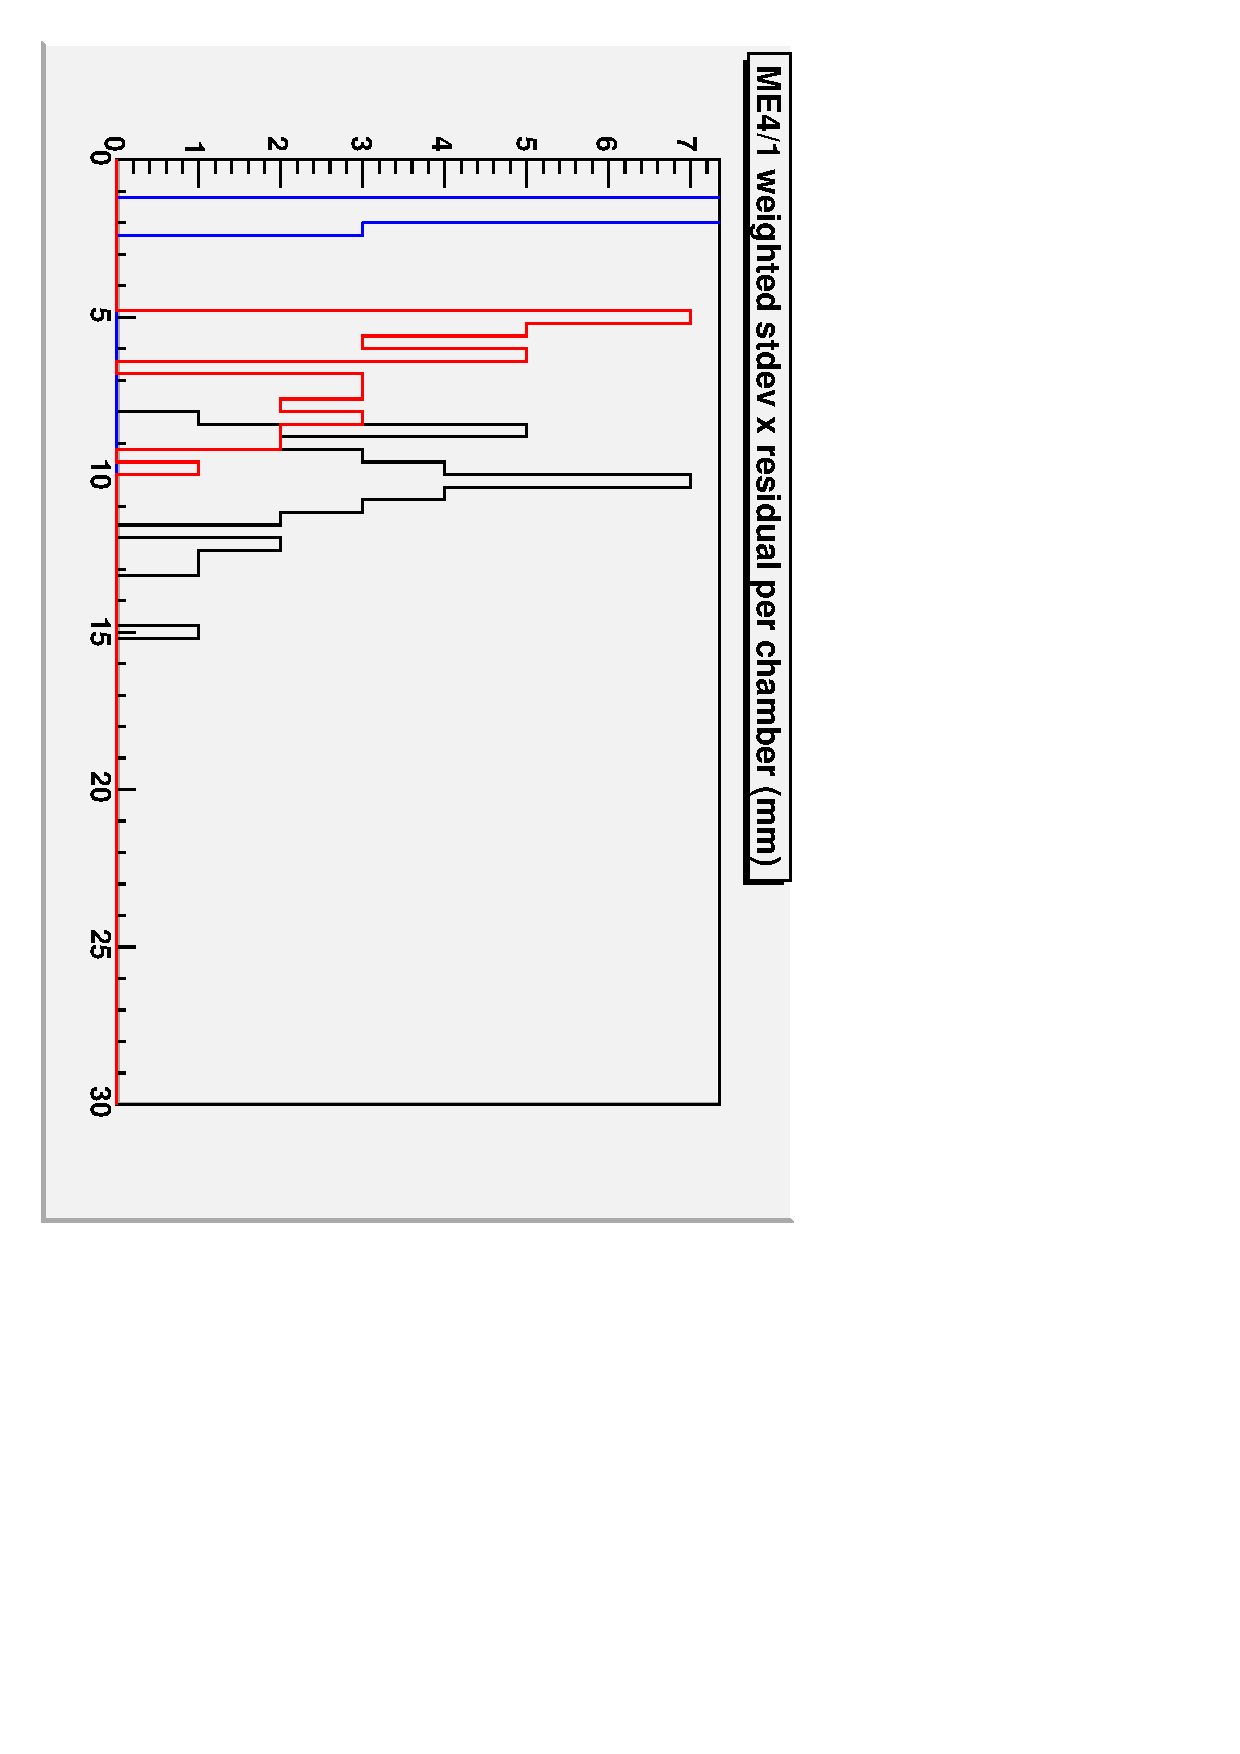
\includegraphics[height=\linewidth, angle=90]{stdevs_me41.pdf}
\end{columns}

\label{numpages}
\end{frame}

\end{document}
